\chapter{Results}

This chapter will present the results that emerged by deploying the previously introduced experiments. We will start with the results from the 3D-Mammoth dataset. Those results are then additionally compared with the results from the transformed 3D-Mammoth dataset. After that, the results from the COIL-20 dataset will be presented. Lastly, we will look into reoccurring phenomena and give insight into the knowledge that we could derive from those experiments.

\section{3D-Mammoth}

This section will deal with the 3D-Mammoth dataset and is divided into subsections that one can also find in Section \ref{sec:exp.prod}.

\subsection{Distance Preservation} \label{subsec:mammoth_dist}

\begin{table}[]
\centering
\begin{tabular}{|c|cl|cc|cc|}
\hline
 & \multicolumn{2}{c|}{{\color[HTML]{1b9e77} \textbf{MDS}}} & \multicolumn{2}{c|}{{\color[HTML]{d95f02} \textbf{LLE}}} & \multicolumn{2}{c|}{{\color[HTML]{7570B3} \textbf{t-SNE}}} \\ \hline
Rank & \multicolumn{2}{c|}{Frob. norm} & \multicolumn{1}{c|}{Param.} & Frob. norm & \multicolumn{1}{c|}{Param.} & Frob. norm \\ \hline
1 & \multicolumn{2}{c|}{\multirow{7}{*}{249}} & \multicolumn{1}{c|}{2463} & 550 & \multicolumn{1}{c|}{9736} & 573 \\ \cline{1-1} \cline{4-7} 
2 & \multicolumn{2}{c|}{} & \multicolumn{1}{c|}{9998} & 552 & \multicolumn{1}{c|}{9740} & 573 \\ \cline{1-1} \cline{4-7} 
3 & \multicolumn{2}{c|}{} & \multicolumn{1}{c|}{9997} & 553 & \multicolumn{1}{c|}{9732} & 573 \\ \cline{1-1} \cline{4-7} 
.. & \multicolumn{2}{c|}{} & \multicolumn{1}{c|}{..} & .. & \multicolumn{1}{c|}{..} & .. \\ \cline{1-1} \cline{4-7} 
9996 & \multicolumn{2}{c|}{} & \multicolumn{1}{c|}{7} & 3431 & \multicolumn{1}{c|}{9772} & 3416 \\ \cline{1-1} \cline{4-7} 
9997 & \multicolumn{2}{c|}{} & \multicolumn{1}{c|}{3} & 3466 & \multicolumn{1}{c|}{9929} & 3420 \\ \cline{1-1} \cline{4-7} 
9998 & \multicolumn{2}{c|}{} & \multicolumn{1}{c|}{5} & 3480 & \multicolumn{1}{c|}{9932} & 3447 \\ \hline
\end{tabular}
\caption[3D-Mammoth Distance Preservation]{Best and worst results from 3D-Mammoth concerning the distance preservation.}
\label{tab:best_worst_dist_mammoth}
\end{table}

\begin{figure}[!]
	\centering
	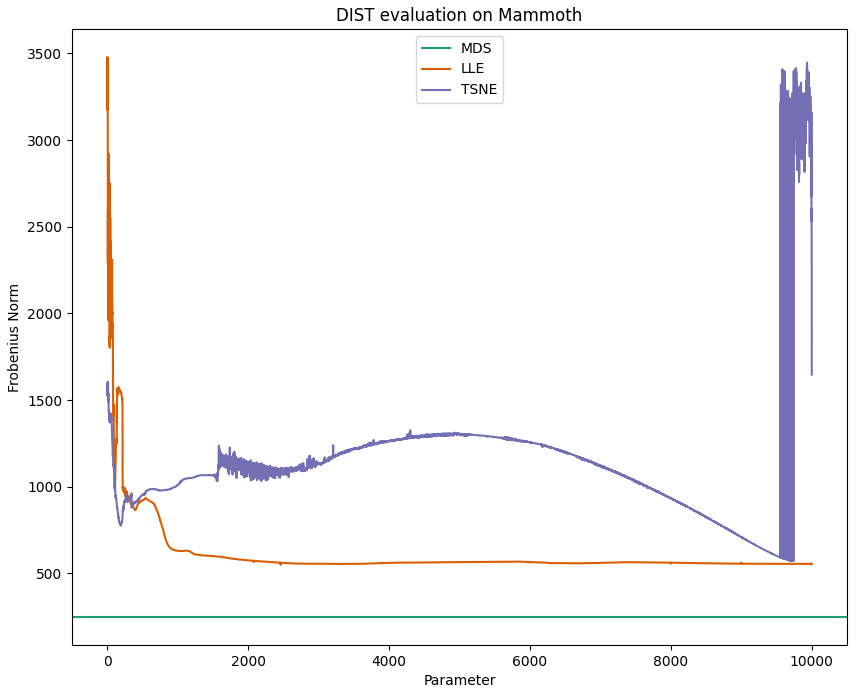
\includegraphics[width=1\columnwidth]{images/DIST_MAMM_all.png}
	\caption[3D-Mammoth Distance Preservation]{Plot showing the distance preservation capability of MDS, LLE, and t-SNE with different parameter settings. Note: MDS has no parameter.}
    \label{fig:best_worst_dist_mammoth}
\end{figure}

By looking at Figure \ref{fig:best_worst_dist_mammoth} and the associated Table \ref{tab:best_worst_dist_mammoth} which show the capability of distance preservation at different parameter settings, one can see that MDS performs best although it has no parameter that can be set. LLE performs second best and t-SNE third. These statements hold not only by looking at the single best parameter setting with its Frobenius norm but also for most of the parameters. On low parameter settings, LLE performs very weakly but the performance gets rapidly better as it reaches more or less a plateau of good results at around $p\leq 2000$. T-SNE however performs well at low parameters (around $p=197$) and then gets weaker with increasing parameters and then gets better again. Finally, at very high parameter settings ($p>9550$), t-SNE arrives at a very unstable stage where it oscillates between the best and the worst embeddings, which we will elaborate on in \ref{sec:rec_phen}. Furthermore, in the graph of LLE, we observe kinks/outliers at some parameter settings which we will elaborate on in \ref{sec:rec_phen}. Interestingly these kinks/outliers do not always result in bad performances but in better ones e.g. at $p=2463$ which also yielded the best distance preservation result.

\subsection{Neighborhood Preservation}

\begin{table}[]
\centering
\begin{tabular}{|c|cl|cc|cc|}
\hline
 & \multicolumn{2}{c|}{{\color[HTML]{1B9E77} \textbf{MDS}}} & \multicolumn{2}{c|}{{\color[HTML]{D95F02} \textbf{LLE}}} & \multicolumn{2}{c|}{{\color[HTML]{7570B3} \textbf{t-SNE}}} \\ \hline
Rank & \multicolumn{2}{c|}{Trust.} & \multicolumn{1}{c|}{Param.} & Trust. & \multicolumn{1}{c|}{Param.} & Trust. \\ \hline
1 & \multicolumn{2}{c|}{} & \multicolumn{1}{c|}{101} & 0.980 & \multicolumn{1}{c|}{2} & 1.000 \\ \cline{1-1} \cline{4-7} 
2 & \multicolumn{2}{c|}{} & \multicolumn{1}{c|}{102} & 0.980 & \multicolumn{1}{c|}{3} & 1.000 \\ \cline{1-1} \cline{4-7} 
3 & \multicolumn{2}{c|}{} & \multicolumn{1}{c|}{100} & 0.980 & \multicolumn{1}{c|}{4} & 1.000 \\ \cline{1-1} \cline{4-7} 
.. & \multicolumn{2}{c|}{} & \multicolumn{1}{c|}{..} & .. & \multicolumn{1}{c|}{..} & .. \\ \cline{1-1} \cline{4-7} 
1436 & \multicolumn{2}{c|}{} & \multicolumn{1}{c|}{7} & 0.870 & \multicolumn{1}{c|}{9841} & 0.874 \\ \cline{1-1} \cline{4-7} 
1437 & \multicolumn{2}{c|}{} & \multicolumn{1}{c|}{8} & 0.855 & \multicolumn{1}{c|}{9978} & 0.873 \\ \cline{1-1} \cline{4-7} 
1438 & \multicolumn{2}{c|}{\multirow{-7}{*}{0.970}} & \multicolumn{1}{c|}{9} & 0.787 & \multicolumn{1}{c|}{9811} & 0.862 \\ \hline
\end{tabular}
\caption[3D-Mammoth Neighborhood Preservation]{Best and worst results from 3D-Mammoth concerning the neighborhood preservation.}
\label{tab:best_worst_1nn_mammoth}
\end{table}

\begin{figure}[!]
	\centering
	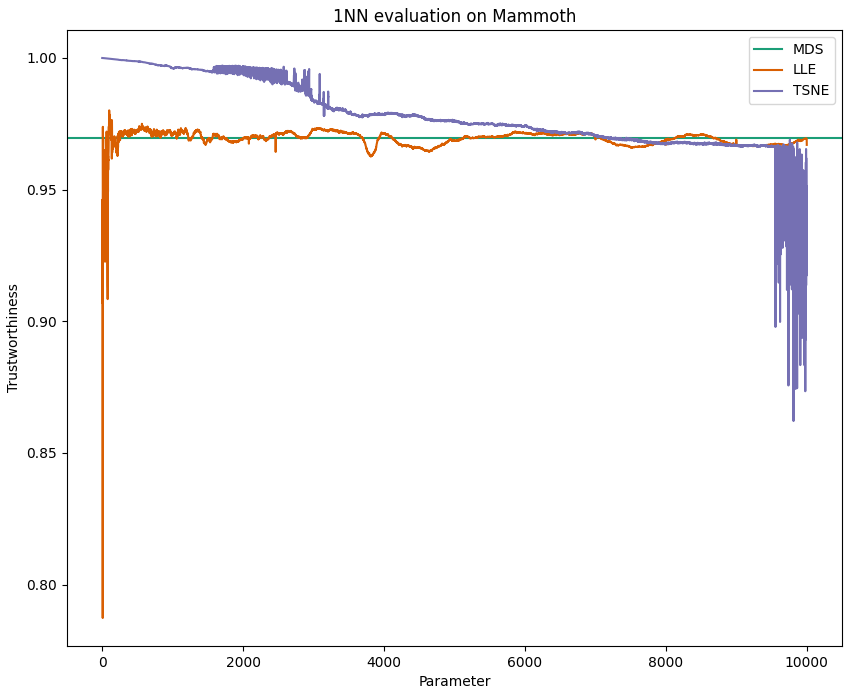
\includegraphics[width=1\columnwidth]{images/1NN_MAMM_all.png}
	\caption[3D-Mammoth Neighborhood Preservation]{Plot showing the neighborhood preservation capability of MDS, LLE, and t-SNE with different parameter settings. Note: MDS has no parameter.}
    \label{fig:1NN_MAMM_all}
\end{figure}

By looking at Figure \ref{fig:1NN_MAMM_all} and the associated Table \ref{tab:best_worst_1nn_mammoth} which show the capability of neighborhood preservation at different parameter settings one can see that t-SNE performs best in terms of best single parameter and across most parameters. The second best single parameter is from a computation of LLE but it is just slightly higher than MDS's computation. As we have seen in Subsection \ref{subsec:mammoth_dist} LLE also performs very weak on low parameter settings but again rapidly doing well again as the parameters get higher. At around $p\leq 100$ LLE starts to reach a plateau and oscillates around the value as MDS. T-SNE on the other hand performs best at low parameter settings but then gets progressively worse as the parameter settings get higher and again reaches an unstable state at $p\leq 9550$.

\subsection{Visualization Quality} \label{subsec:visqual_mamoth}

\begin{figure}[!]
     \centering
     \begin{subfigure}[t]{0.51\columnwidth}
    	\centering
    	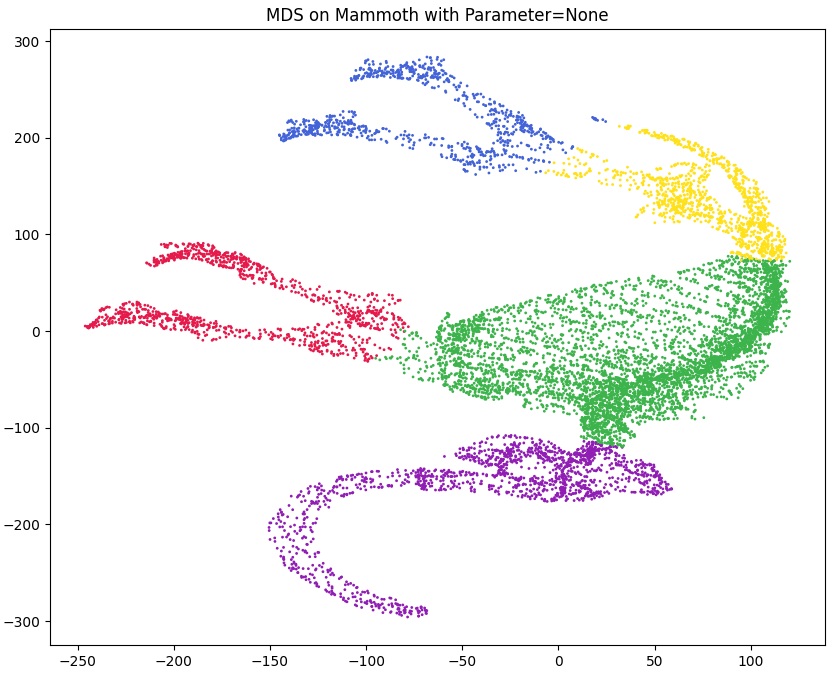
\includegraphics[width=\columnwidth]{images/mammoth_mds_plot.png}
    	\caption{MDS}
        \label{fig:mammoth_mds_plot}
    \end{subfigure}
     \hfill
     \begin{subfigure}[t]{0.49\columnwidth}
    	\centering
    	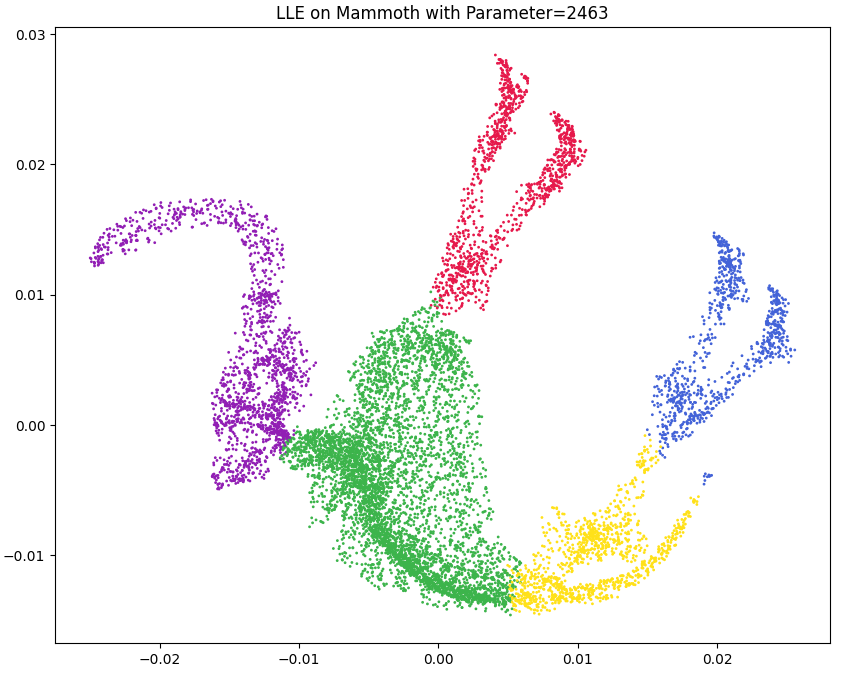
\includegraphics[width=\columnwidth]{images/mammoth_lle2463_plot.png}
    	\caption{LLE result with $p=2463$}
        \label{fig:mammoth_lle2463_plot}
    \end{subfigure}
     \hfill
     \begin{subfigure}[t]{0.49\columnwidth}
    	\centering
    	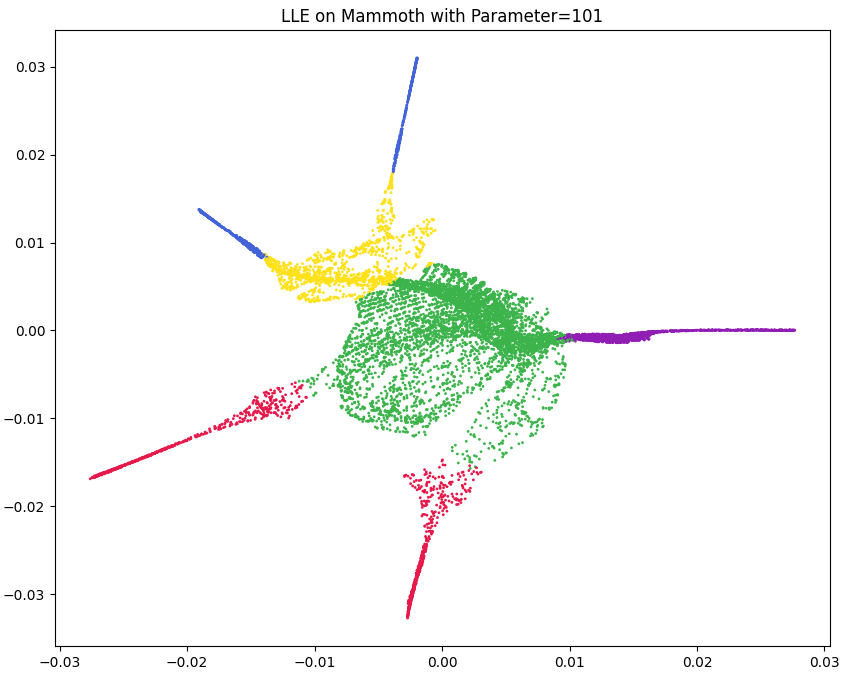
\includegraphics[width=\columnwidth]{images/mammoth_lle101_plot.png}
    	\caption{LLE with $p=101$}
        \label{fig:mammoth_lle101_plot}
    \end{subfigure}
     \hfill
     \begin{subfigure}[t]{0.49\columnwidth}
    	\centering
    	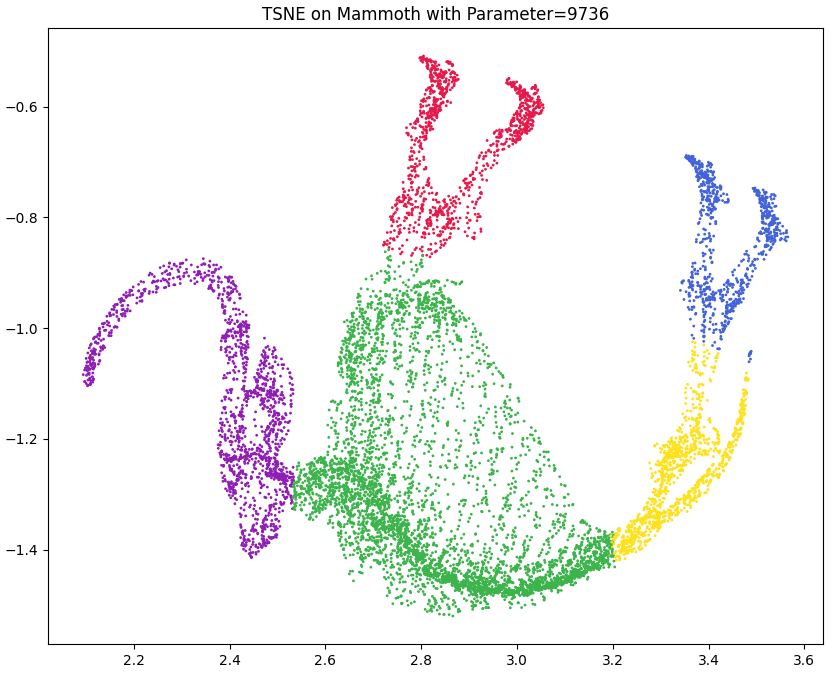
\includegraphics[width=\columnwidth]{images/mammoth_tsne9736_plot.png}
    	\caption{t-SNE with $p=9736$}
        \label{fig:mammoth_tsne9736_plot}
    \end{subfigure}
     \hfill
     \begin{subfigure}[t]{0.49\columnwidth}
    	\centering
    	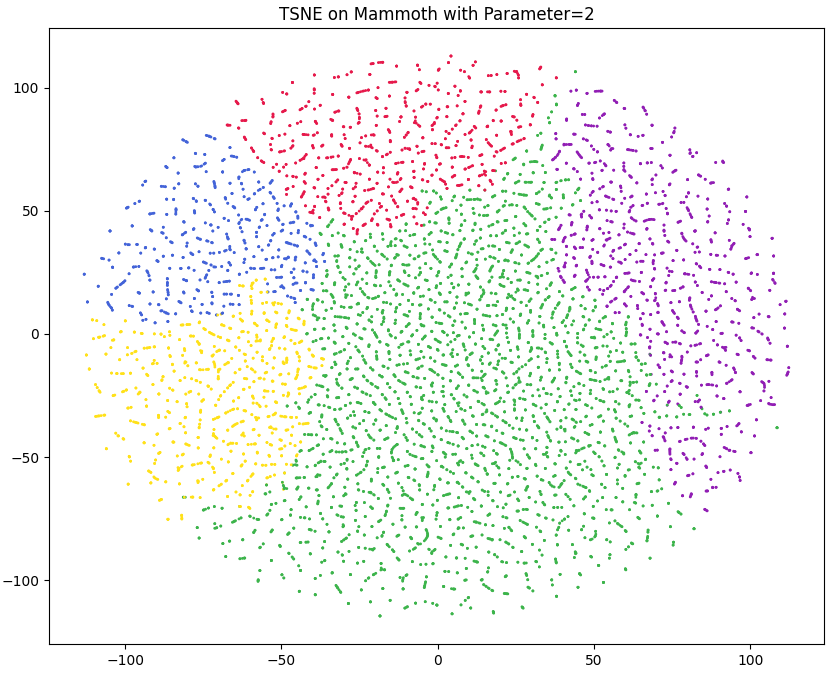
\includegraphics[width=\columnwidth]{images/mammoth_tsne2_plot.png}
    	\caption{t-SNE with $p=2$}
        \label{fig:mammoth_tsne2_plot}
    \end{subfigure}
     \caption[3D-Mammoth Visualisations of Best Results]{Visualizations of best mammoth distance (left) and neighborhood (right) preservation results. Note: There is only a single visualization of MDS.}
    \label{fig:mammoth_visual_best}
\end{figure}

By comparing the visualizations of the best results emerging from the distance preservation (left column at Figure \ref{fig:mammoth_visual_best}) one could come to the conclusion that the best visualization is derived from LLE (Subfigure \ref{fig:mammoth_lle2463_plot}). We come to this conclusion because this visualization looks most appealing to the human eye as it firstly clearly represents a side view of a mammoth and among the best visualizations which include MDS (Subfigure \ref{fig:mammoth_mds_plot}) and t-SNE with $p=9736$ (Subfigure \ref{fig:mammoth_tsne9736_plot}) it is the most balanced one, meaning it comes very close to the original proportions of the 3D-Mammoth dataset. The other good visualizations seem to be stretched and/or have an oversized rib cage.

Further, by comparing the visualizations of the best results emerging from the neighborhood preservation (right column at Figure \ref{fig:mammoth_visual_best}) one could come to the conclusion that the best visualization is derived from MDS (Subfigure \ref{fig:mammoth_mds_plot}), although the embedding seems to be a little bit stretched. The best result from LLE concerning the neighbored preservation (Subfigure \ref{fig:mammoth_lle101_plot}) resulted in a visualization where the torso was embedded pretty well because one can easily distinguish the spine and the ribs, but the extremities were embedded in a straight line. The visualization of the best neighborhood preservation of t-SNE with $p=2$ (Subfigure \ref{fig:mammoth_tsne2_plot}) is from a visualization quality standpoint very bad as it does not represent a mammoth in any form but it shows us that by embedding all data points into a continuous blob one can easily preserve the 1-neighborhoods.

Note that although t-SNE with $p=2$ ($trust.=1$) and LLE with $p=101$ ($trust.=0.98$) have better neighborhood preservation than MDS ($trust.=0.97$), MDS has the best visualization of those. This circumstance gives a hint that good neighborhood preservation does not imply good visualization quality. This can further be verified if we look at Figure \ref{fig:visualisation_quality} which illustrates that good distance preservation also does not imply a good visualization quality.

\begin{figure}[!]
     \centering
     \begin{subfigure}[t]{0.49\columnwidth}
    	\centering
    	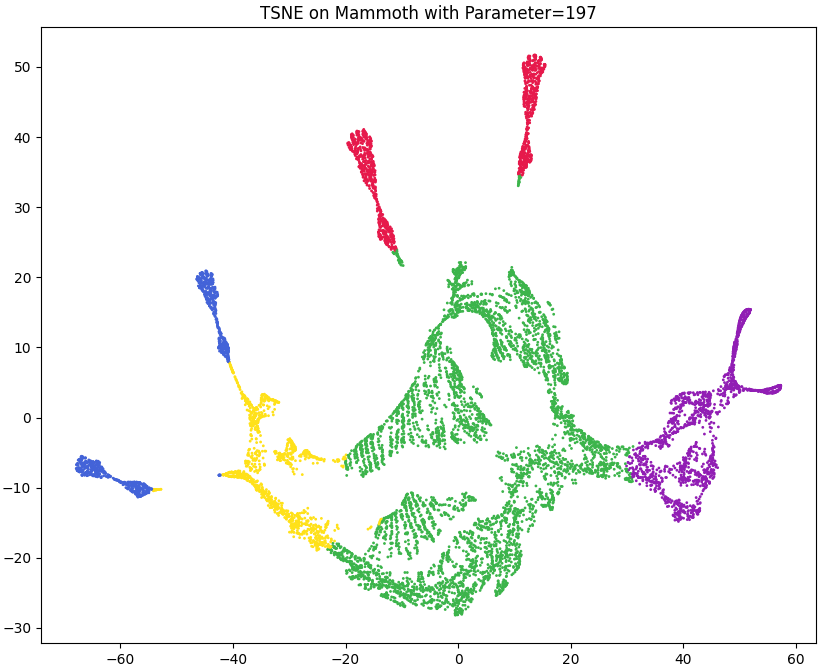
\includegraphics[width=\columnwidth]{images/mammoth_tsne197_plot.png}
    	\caption{t-SNE with $p=197$ and $Frob. norm=776$}
        \label{fig:mammoth_tsne197_plot}
    \end{subfigure}
     \hfill
     \begin{subfigure}[t]{0.49\columnwidth}
    	\centering
    	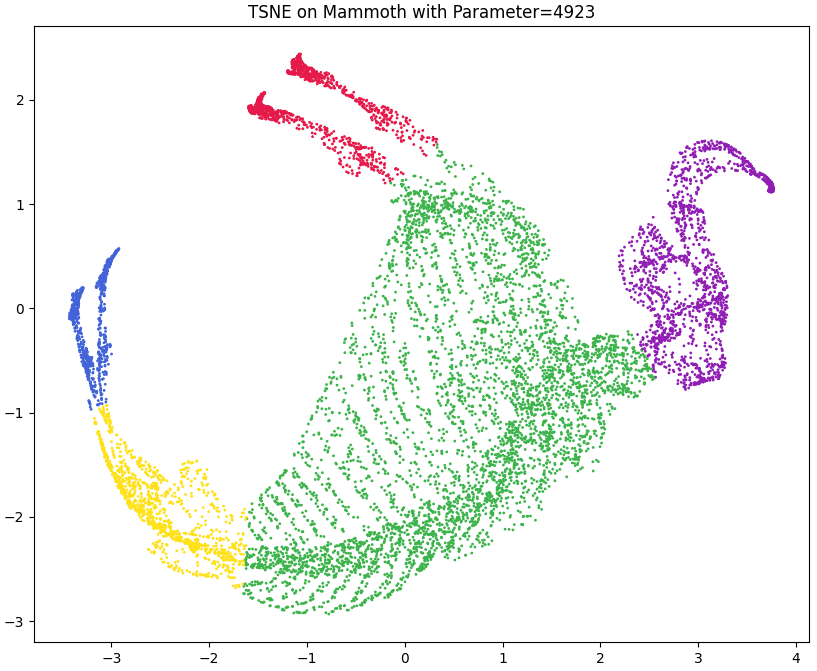
\includegraphics[width=\columnwidth]{images/mammoth_tsne4923_plot.png}
    	\caption{t-SNE with $p=4923$ and $Frob. norm=1312$}
        \label{fig:mammoth_tsne4923_plot}
    \end{subfigure}
     \caption[Visualisation Quality of Embeddings]{These plots show us that good distance preservation does not imply a good visualization quality. Left: bad vis. quality and good dist. preservation, Right: good vis. quality and bad dist. preservation.}
    \label{fig:visualisation_quality}
\end{figure}

\begin{figure}[!]
     \centering
     \begin{subfigure}[t]{0.49\columnwidth}
    	\centering
    	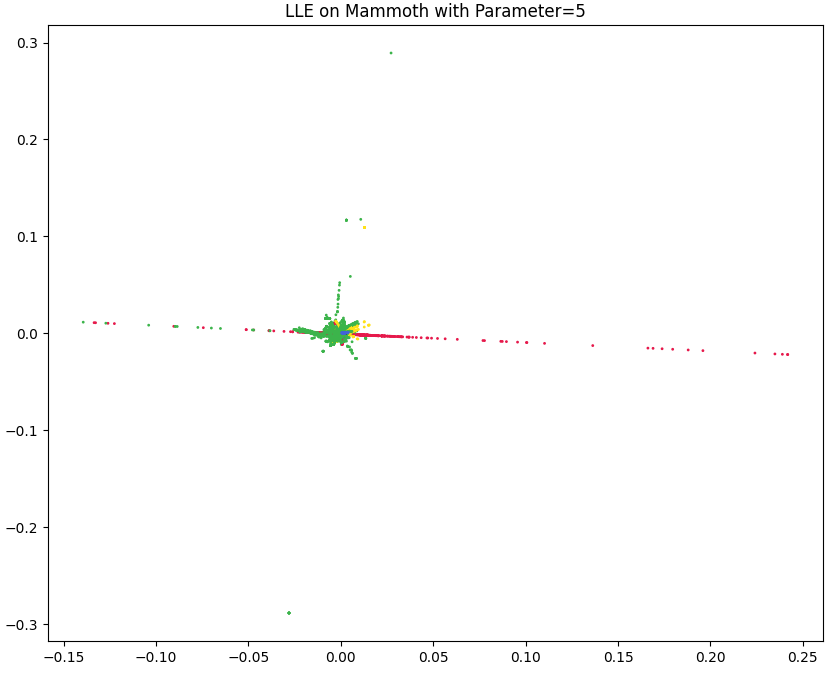
\includegraphics[width=\columnwidth]{images/mammoth_lle5_plot.png}
    	\caption{LLE with $p=5$ (worst dist. preservation)}
        \label{fig:mammoth_lle5_plot}
    \end{subfigure}
     \hfill
     \begin{subfigure}[t]{0.49\columnwidth}
    	\centering
    	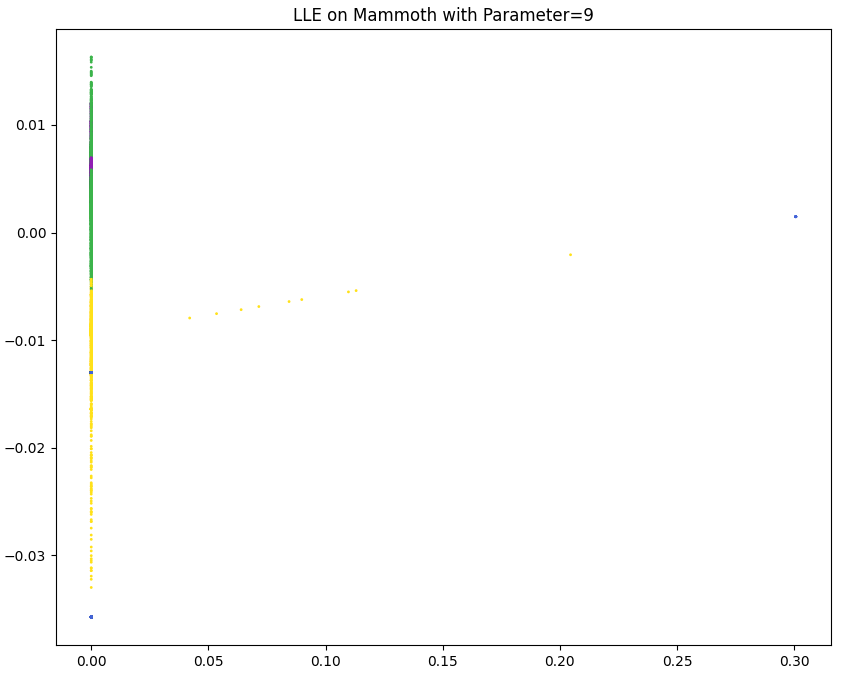
\includegraphics[width=\columnwidth]{images/mammoth_lle9_plot.png}
    	\caption{LLE with $p=9$ (worst neigh. preservation)}
        \label{fig:mammoth_lle9_plot}
    \end{subfigure}
     \caption[Visualization of Worst LLE Results]{Visualizations of the worst LLE results.}
    \label{fig:lle_worst_vis}
\end{figure}

The visualization of the worst distance and neighborhood preservation (Figure \ref{fig:lle_worst_vis} shows us that LLE tends to collapse into some points which can be seen in the fact that the whole embedding is in a small 2-dimensional space (low values for x- and y- axis) and tries to compensate the optimization function by embedding other points as well as possible. One notices that LLE somehow detects related structures (clusters) such as the mammoth rib cage or back and tail and embeds these well compared to other structures which results in a straight line.

\begin{figure}[!]
     \centering
     \begin{subfigure}[t]{0.49\columnwidth}
    	\centering
    	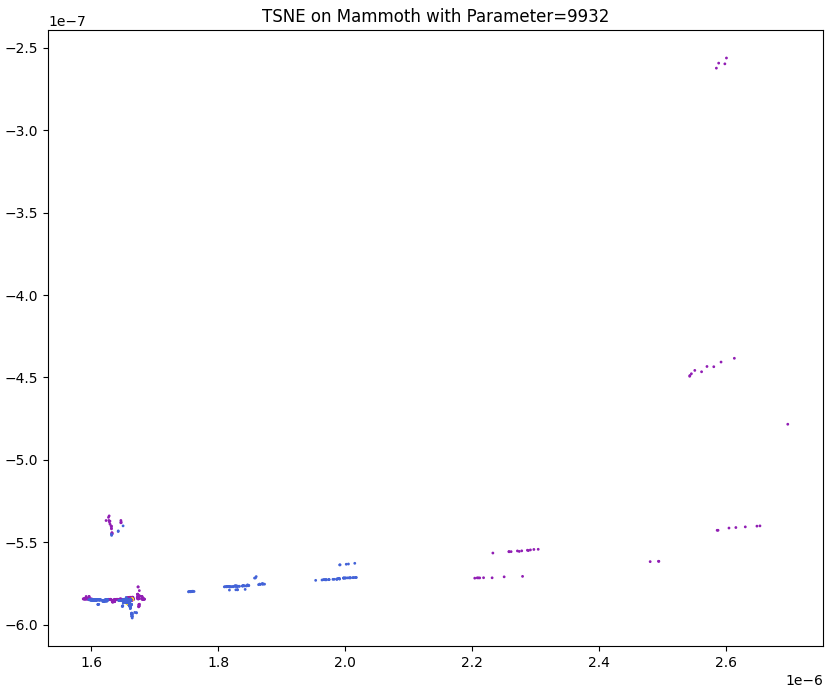
\includegraphics[width=\columnwidth]{images/mammoth_tsne9932_plot.png}
    	\caption{t-SNE with $p=9932$ \\ (worst dist. preservation)}
        \label{fig:mammoth_tsne9932_plot}
    \end{subfigure}
     \hfill
     \begin{subfigure}[t]{0.49\columnwidth}
    	\centering
    	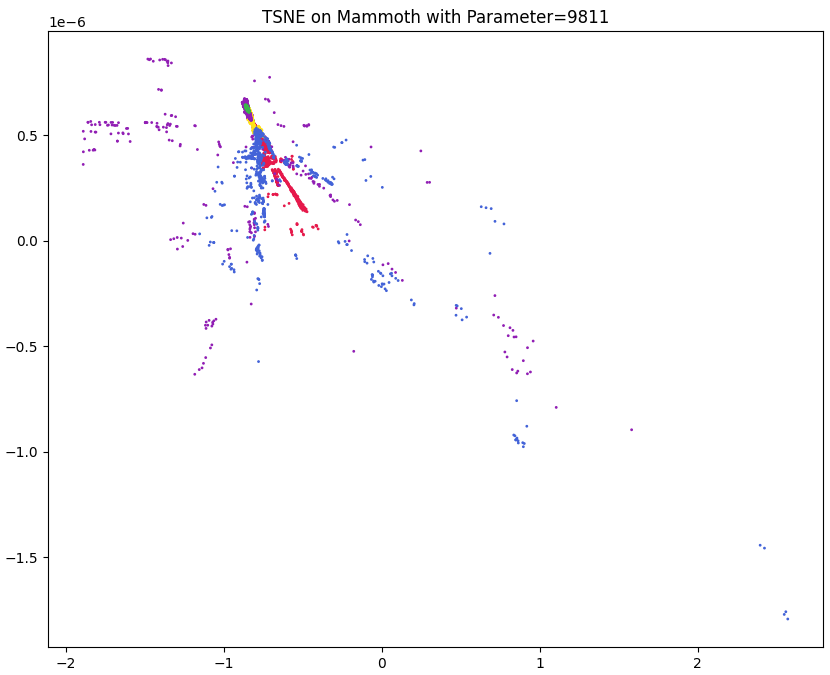
\includegraphics[width=\columnwidth]{images/mammoth_tsne9811_plot.png}
    	\caption{t-SNE with $p=9811$ \\ (worst neigh. preservation)}
        \label{fig:mammoth_tsne9811_plot}
    \end{subfigure}
     \caption[Visualization of Worst t-SNE Results]{Visualizations of the worst t-SNE results.}
    \label{fig:tsne_worst_vis}
\end{figure}

In Figure \ref{fig:tsne_worst_vis} one can see the worst results for t-SNE which show a similar behavior in that the embedding collapsed into a very small space, even smaller than LLE's embedding. The difference to LLE's worst results is that t-SNE does not favor the correct embedding of specific regions/body parts. Instead, it preserves the neighborhoods and distances for all points equally bad.

Another approach to get more insight into which structures of the 3D-Mammoth are embedded well or badly is by creating a heatmap on the high-dimensional Mammoth (introduced in \ref{subsec:vis_qual}). Figure \ref{fig:heat_mamm} shows the best and worst embeddings of all manifold learning methods. The first heatmap shows us impressively how MDS actually works, at least on this dataset. The mammoth is shown from above and all datapoints in a straight line from left to right are embedded perfectly and the more you get to the top or bottom the more points are getting less good distance preservation values. This means that MDS, in this case, just constructed a 2-dimensional plane in the middle of the mammoth and embedded all points onto it. This behavior probably can be seen in various linear dimensionality reduction methods such as PCA. Further, the worst embeddings of LLE and t-SNE are such that the center of the mammoth was embedded well but the more you go from the center of the body away the points are increasingly worse embedded. This can be explained by the fact that if an embedding is collapsing, which is the case in the worst tries of LLE and t-SNE, then those points in high dimensional space that have the least average distance to all other points are theoretically best preserves. Points at the outside, here at the extremities have a high average distance to all other points, and therefore it seems as if there is a pattern. However, this pattern occurs naturally if the embedding collapses. Nonetheless, we can not explain why in the worst embedding of t-SNE there are points on the back feet, seemingly lying on a line/plane, that are embedded a lot better than the adjacent points. Further, in the good LLE embeddings, there was a pattern that could be observed. We chose to just present the best one but all other good embeddings follow a similar pattern. There the embedding did well in preserving the distances of all points but the front feet. This must therefore be a peculiarity of LLE which we cannot explain. Note that the value range in this case is very low meaning that the front feet were embedded very well but in comparison to all other points they are bad. The interesting part of the heatmap of the best and all other good t-SNE embeddings is that there is a different pattern that emerges where the extremities are mostly very well preserved but the center of the body, except for one patch, is preserved a little bit worse. Those behaviors we cannot explain yet, therefore further research must be condcuted.

\begin{figure}[!]
     \centering
     \begin{subfigure}[t]{0.51\columnwidth}
    	\centering
    	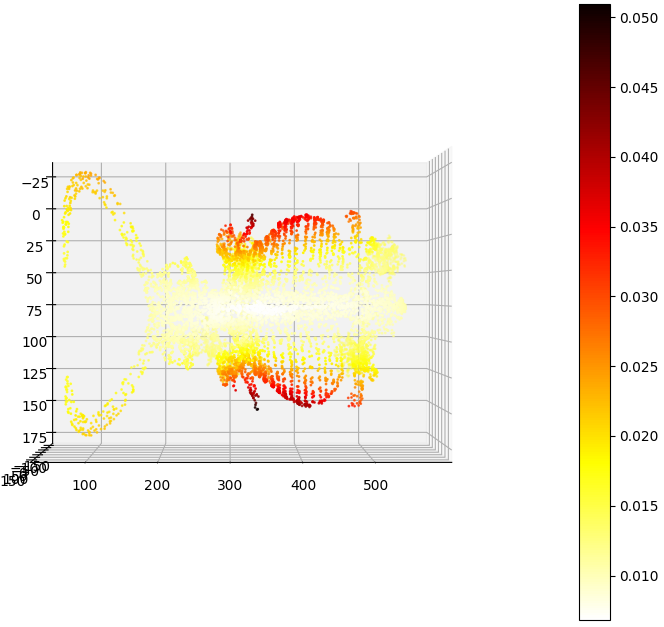
\includegraphics[width=\columnwidth]{images/reverse_mds_mammoth.png}
    	\caption{MDS, imaged from above.}
        \label{fig:reverse_mds_mammoth}
    \end{subfigure}
     \hfill
     \begin{subfigure}[t]{0.49\columnwidth}
    	\centering
    	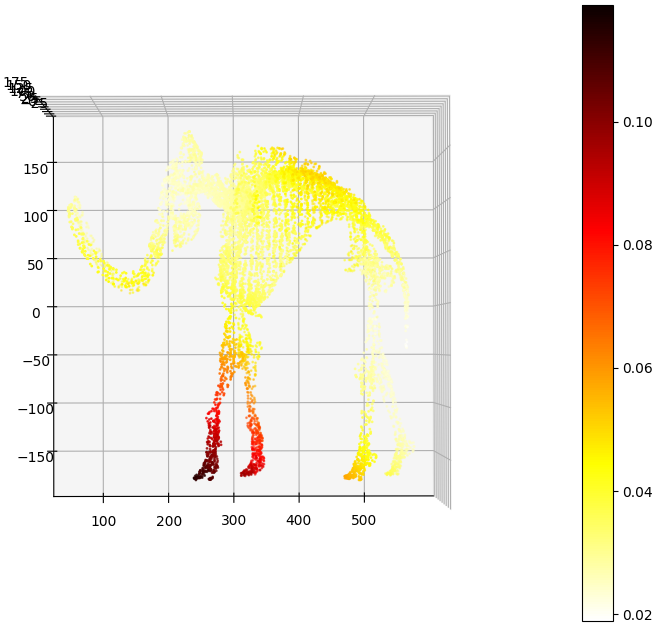
\includegraphics[width=\columnwidth]{images/reverse_best_lle_mammoth.png}
    	\caption{Best LLE embedding \\ with $p=2463$}
        \label{fig:reverse_best_lle_mammoth}
    \end{subfigure}
     \hfill
     \begin{subfigure}[t]{0.49\columnwidth}
    	\centering
    	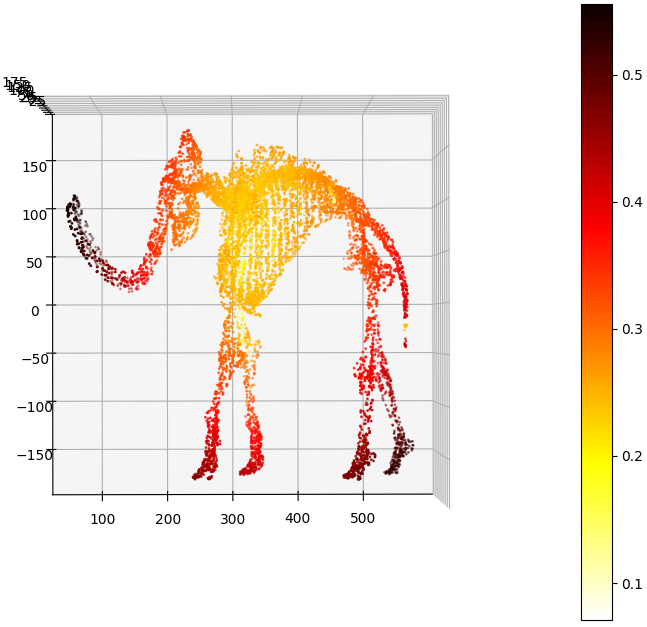
\includegraphics[width=\columnwidth]{images/reverse_worst_lle_mammoth.png}
    	\caption{Worst LLE embedding \\ with $p=5$}
        \label{fig:reverse_worst_lle_mammoth}
    \end{subfigure}
     \hfill
     \begin{subfigure}[t]{0.49\columnwidth}
    	\centering
    	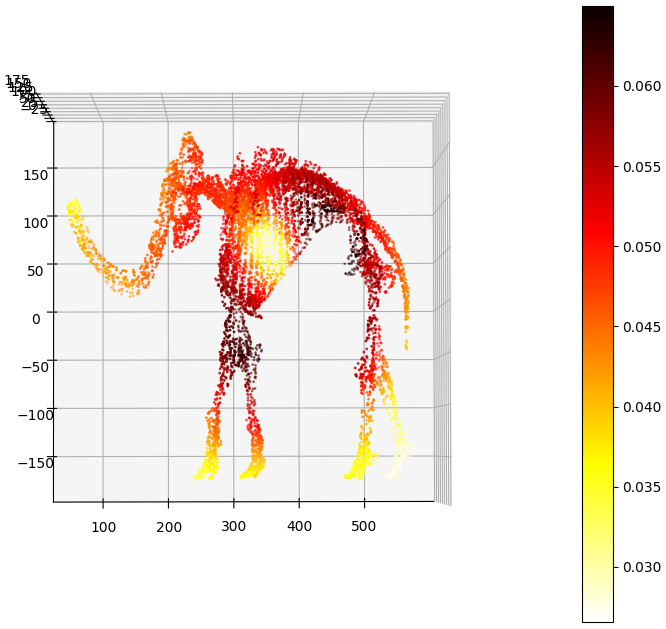
\includegraphics[width=\columnwidth]{images/reverse_best_tsne_mammoth.png}
    	\caption{Best t-SNE embedding \\ with $p=9736$}
        \label{fig:reverse_best_tsne_mammoth}
    \end{subfigure}
     \hfill
     \begin{subfigure}[t]{0.49\columnwidth}
    	\centering
    	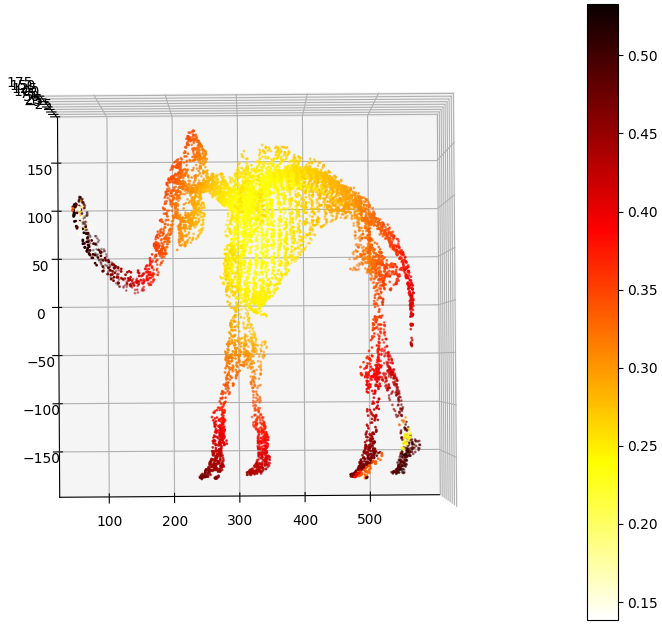
\includegraphics[width=\columnwidth]{images/reverse_worst_tsne_mammoth.png}
    	\caption{Worst t-SNE embedding \\ with $p=9932$}
        \label{fig:reverse_worst_tsne_mammoth}
    \end{subfigure}
     \caption[Heatmaps of 3D-Mammoth Distance Preservations]{Heatmaps of the distance preservation tries on 3D-Mammoth. Note: The colormaps are not normalized and therefore differ in the value ranges.}
    \label{fig:heat_mamm}
\end{figure}

\subsection{Clusterability on Embeddings} \label{subsec:clu_mamm}

For evaluating the clusterability of the low dimensional embedding of the Mammoth dataset we first calculated the silhouette scores of clustering results by deploying $k$-Means with different $k$. The best clustering according to the silhouette score can be seen in Figure \ref{fig:KMEANS_MAMMOTH_5}. For the upper limit of $k$, we chose $\frac{1}{3}$ of the number of data points because everything above is most likely not relevant for real-world examples. Another reason is that, we have already seen in the course of the graph to the complete silhouette score evaluation on the high dimensional COIL-20 dataset (Figure \ref{fig:SC_KMEANS_COIL20_high}) that the higher the number of clusters gets the lower the silhouette score gets. We suspected that the same would happen here.

\begin{figure}[!]
	\centering
	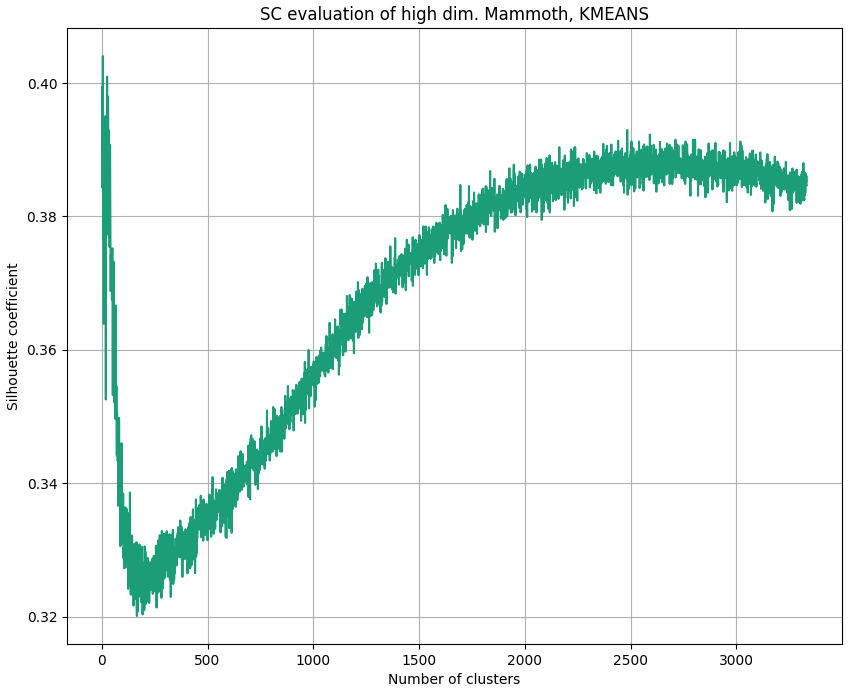
\includegraphics[width=0.85\columnwidth]{images/SC_KMEANS_MAMMOTH.png}
	\caption[Silhouette Scores for 3D-Mammoth]{Silhouette scores of high dimensional 3D-Mammoth dataset after deploying $k$-Means with $2\leq k \leq 3333$.}
    \label{fig:SC_KMEANS_MAMMOTH}
\end{figure}

\begin{figure}[!]
	\centering
	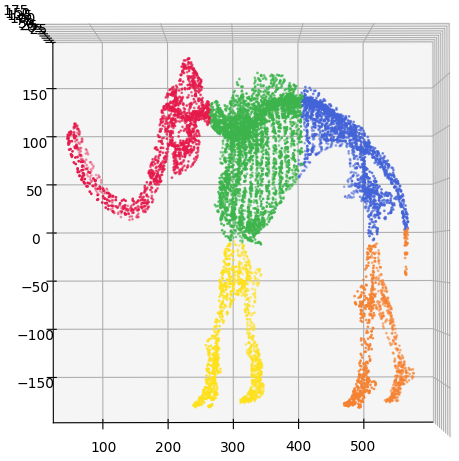
\includegraphics[width=0.5\columnwidth]{images/KMEANS_MAMMOTH_5.png}
	\caption[Visualisation of Best Clustering on 3D-Mammoth]{Visualisation of the best $k$-Means clustering on 3D-Mammoth with $k=5$, $SC=0.40$.}
    \label{fig:KMEANS_MAMMOTH_5}
\end{figure}

\begin{table}[]
\centering
\begin{tabular}{|c|c|c|c|c|c|c|}
\hline
      & \textbf{Type}            & \textbf{Method}                                         & \textbf{Param.} & \textbf{SC} & \textbf{ARI} & \textbf{AMI} \\ \hline
-     & - & {\color[HTML]{1B9E77} \textbf{MDS}}                   & {\color[HTML]{1B9E77} -} & 0.45 & 0.95 & 0.95 \\ \hline
best  &   & {\color[HTML]{D95F02} }                               & 2463                     & 0.45 & 0.75 & 0.82 \\ \cline{1-1} \cline{4-7} 
worst &   & \multirow{-2}{*}{{\color[HTML]{D95F02} \textbf{LLE}}} & 5                        & 0.93 & 0.00 & 0.01 \\ \cline{1-1} \cline{3-7} 
best  &   & {\color[HTML]{7570B3} }                               & 9736                     & 0.45 & 0.58 & 0.72 \\ \cline{1-1} \cline{4-7} 
worst & \multirow{-4}{*}{global} & \multirow{-2}{*}{{\color[HTML]{7570B3} \textbf{t-SNE}}} & 9932            & 0.97        & 0.01         & 0.04         \\ \hline
best  &   & {\color[HTML]{D95F02} }                               & 101                      & 0.45 & 0.53 & 0.66 \\ \cline{1-1} \cline{4-7} 
worst &   & \multirow{-2}{*}{{\color[HTML]{D95F02} \textbf{LLE}}} & 9                        & 0.82 & 0.23 & 0.38 \\ \cline{1-1} \cline{3-7} 
best  &   & {\color[HTML]{7570B3} }                               & 2                        & 0.32 & 0.21 & 0.39 \\ \cline{1-1} \cline{4-7} 
worst & \multirow{-4}{*}{local}  & \multirow{-2}{*}{{\color[HTML]{7570B3} \textbf{t-SNE}}} & 9811            & 0.78        & 0.16         & 0.23         \\ \hline
\end{tabular}
\caption[Cluster Evaluation on 3D-Mammoth]{Scores for low dimensional Mammoth embeddings with $k=5$.}
\label{tab:clu_mammoth}
\end{table}

By looking at the clustering evaluation results of the low dimensional Mammoth embeddings (Figure \ref{tab:clu_mammoth}) we can observe that every 'worst' embedding had a good ($>0.78$) silhouette score. This is at first counter-intuitive because these embeddings did collapse and do not represent a good embedding. For those embeddings, the corresponding ARI and AMI scores however state that the original clusterings did not match with the found ones in the low-dimensional embeddings. This shows us that the clusters that were found have a good cluster structure in terms of separation and cohesion but are not accurate, even random. The reason for this is that the embedding collapsed which means that the cluster is very tight (high cohesion) which results in a high silhouette score.

The silhouette score of the 'best' embeddings and MDS are at most $0.45$. We suspect that this score is the maximum possible value for the Mammoth dataset because of the continuity property. This property limits the separability of clusters immensely.
By comparing the ARI and the AMI scores of the best local and global embeddings we observe that distance preservation is more likely to preserve the clusterings than neighborhood preservation. Another interesting thing is that of all methods and types the MDS method performed significantly better than every other configuration.

Those who are interested in the visualizations of the low dimensional embeddings corresponding to Table \ref{tab:clu_mammoth} can look these up in Figure \ref{fig:global_clu_mammoth} and \ref{fig:local_clu_mammoth}.

\begin{figure}[!]
     \centering
     \begin{subfigure}[t]{0.51\columnwidth}
    	\centering
    	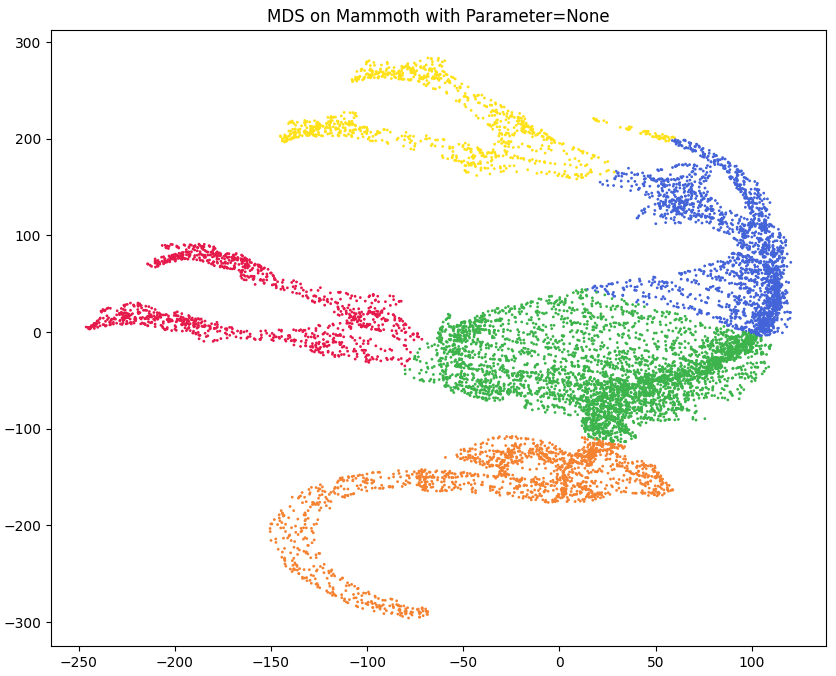
\includegraphics[width=\columnwidth]{images/KMEANS_5_MDS.png}
    	\caption{MDS}
        \label{fig:KMEANS_5_MDS}
    \end{subfigure}
     \hfill
     \begin{subfigure}[t]{0.49\columnwidth}
    	\centering
    	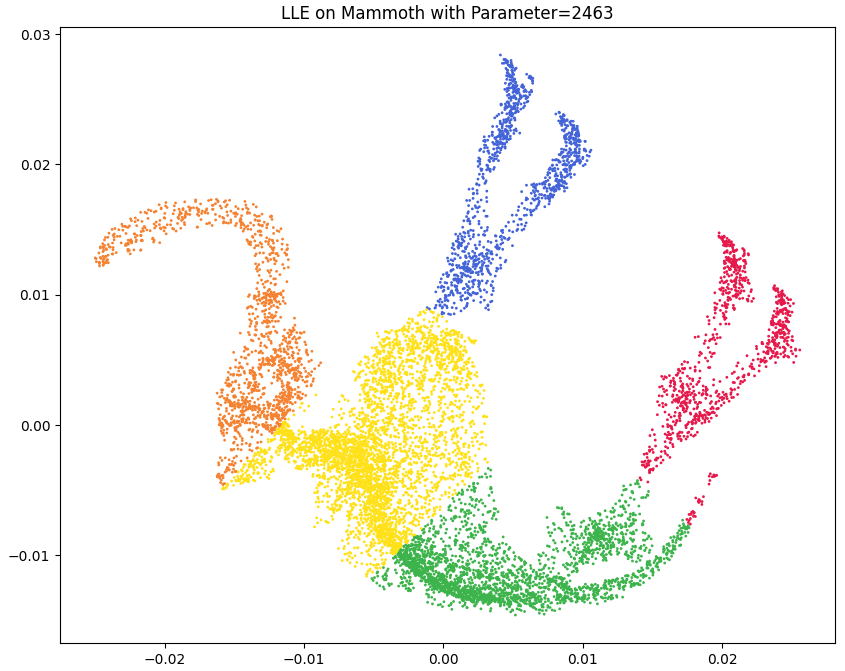
\includegraphics[width=\columnwidth]{images/KMEANS_5_LLE_2463.png}
    	\caption{LLE with $p=2463$}
        \label{fig:KMEANS_5_LLE_2463}
    \end{subfigure}
     \hfill
     \begin{subfigure}[t]{0.49\columnwidth}
    	\centering
    	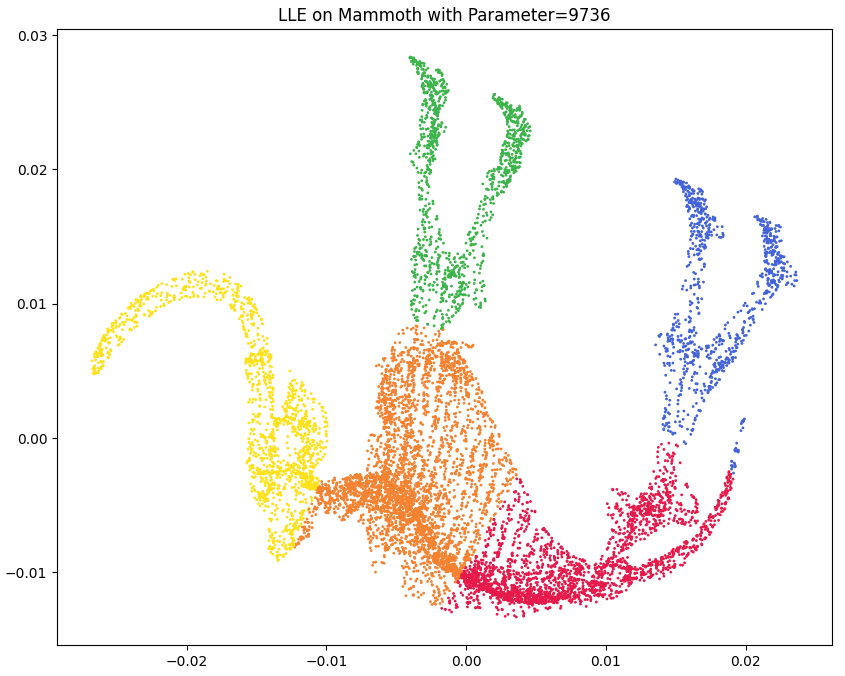
\includegraphics[width=\columnwidth]{images/KMEANS_5_TSNE_9736.png}
    	\caption{t-SNE with $p=9736$}
        \label{fig:KMEANS_5_TSNE_9736}
    \end{subfigure}
    \hfill
     \begin{subfigure}[t]{0.49\columnwidth}
    	\centering
    	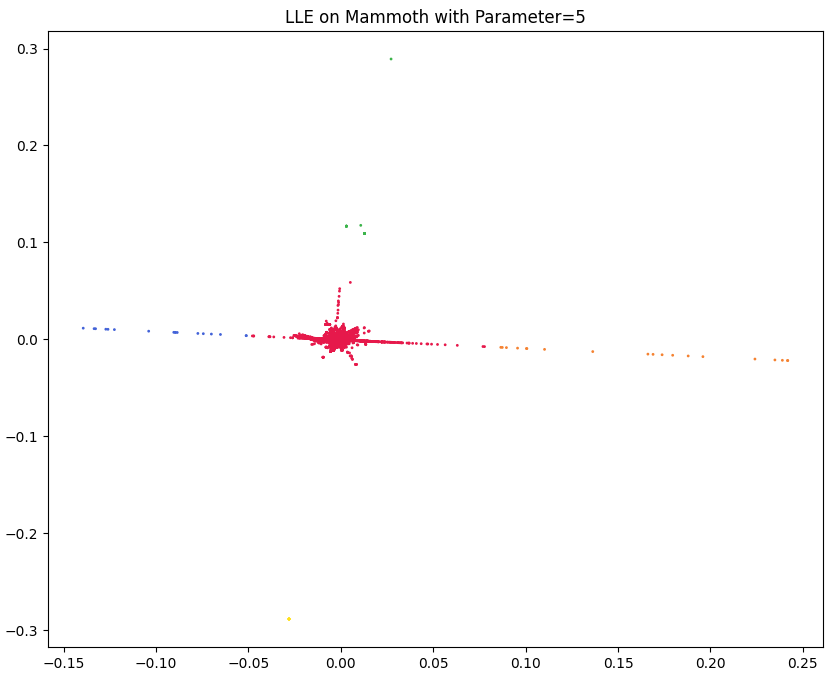
\includegraphics[width=\columnwidth]{images/KMEANS_5_LLE_5.png}
    	\caption{LLE with $k=5$}
        \label{fig:KMEANS_5_LLE_5}
    \end{subfigure}
     \hfill
     \begin{subfigure}[t]{0.49\columnwidth}
    	\centering
    	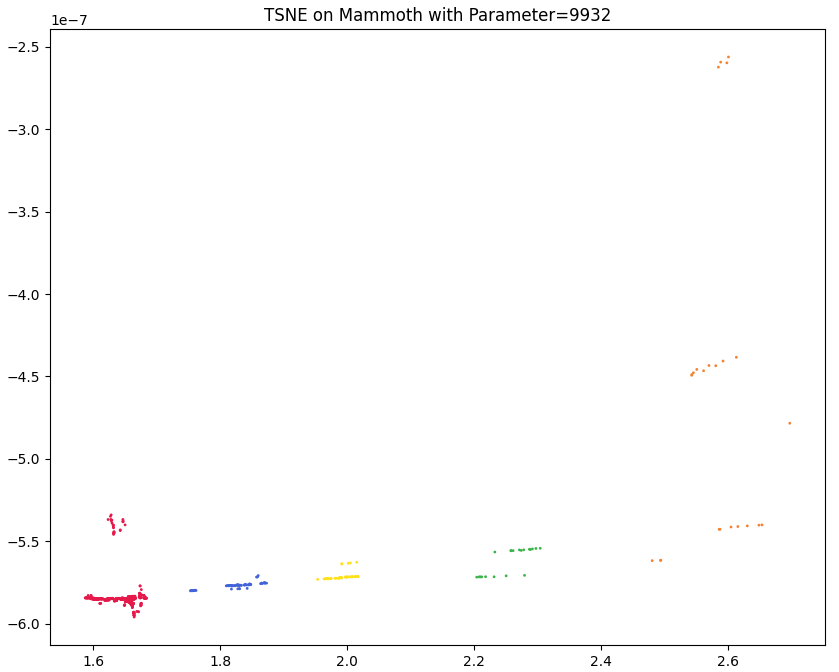
\includegraphics[width=\columnwidth]{images/KMEANS_5_TSNE_9932.png}
    	\caption{t-SNE $k=9932$}
        \label{fig:KMEANS_5_TSNE_9932}
    \end{subfigure}
     \caption[Clusters on low dim. 3D-Mammoth (global)]{Clusters on low dim. 3D-Mammoth (global), corresponding to Table \ref{tab:clu_mammoth}.}
    \label{fig:global_clu_mammoth}
\end{figure}

\begin{figure}[!]
     \centering
     \begin{subfigure}[t]{0.49\columnwidth}
    	\centering
    	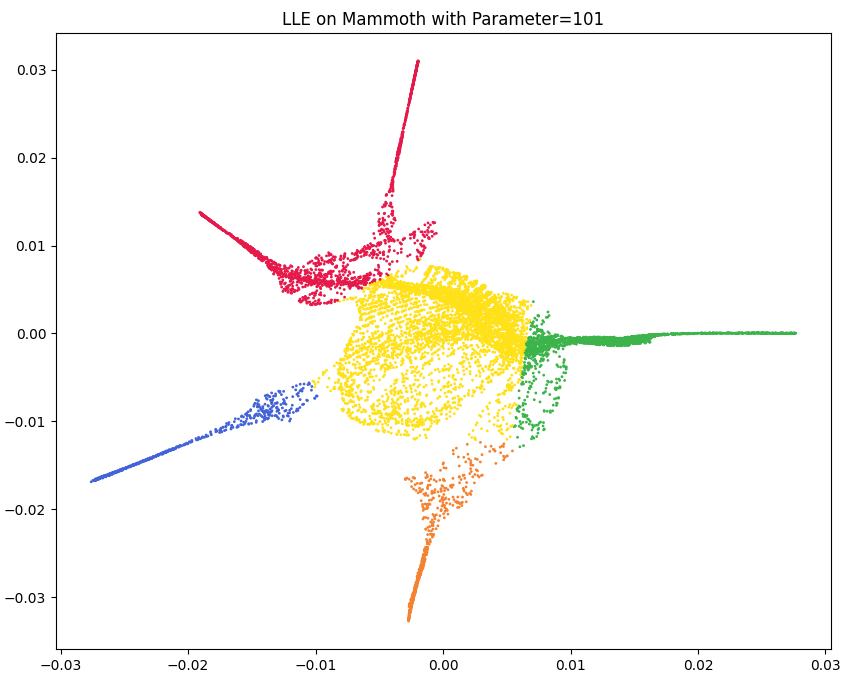
\includegraphics[width=\columnwidth]{images/KMEANS_5_LLE_101.png}
    	\caption{LLE with $p=101$}
        \label{fig:KMEANS_5_LLE_101}
    \end{subfigure}
     \hfill
     \begin{subfigure}[t]{0.49\columnwidth}
    	\centering
    	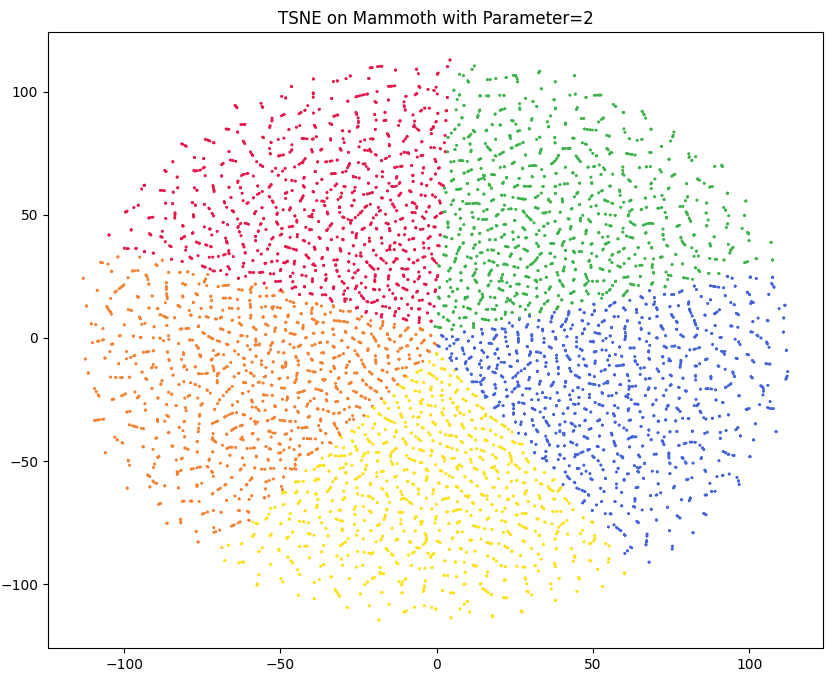
\includegraphics[width=\columnwidth]{images/KMEANS_5_TSNE_2.png}
    	\caption{t-SNE with $p=2$}
        \label{fig:KMEANS_5_TSNE_2}
    \end{subfigure}
    \hfill
     \begin{subfigure}[t]{0.49\columnwidth}
    	\centering
    	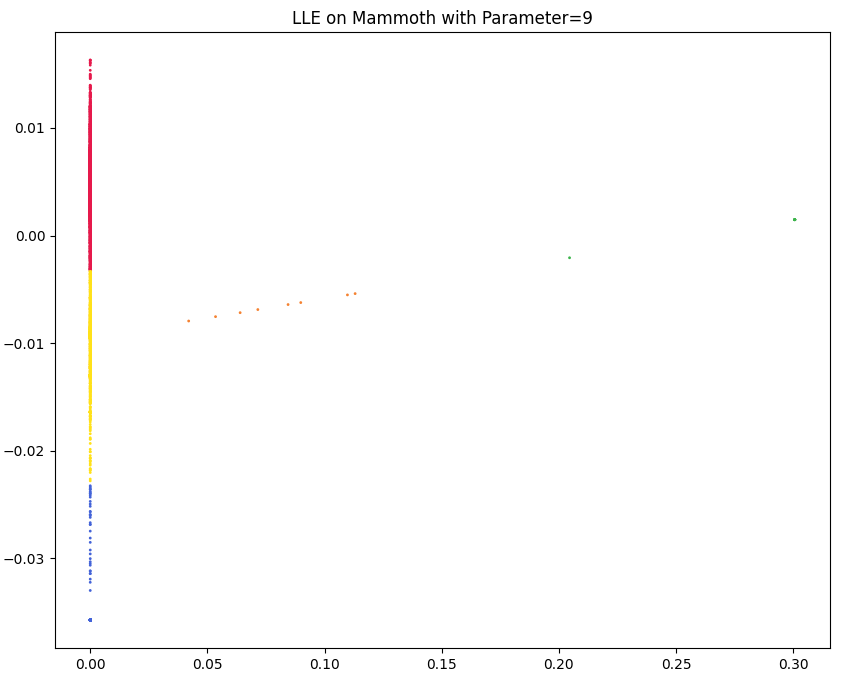
\includegraphics[width=\columnwidth]{images/KMEANS_5_LLE_9.png}
    	\caption{LLE with $k=9$}
        \label{fig:KMEANS_5_LLE_9}
    \end{subfigure}
     \hfill
     \begin{subfigure}[t]{0.49\columnwidth}
    	\centering
    	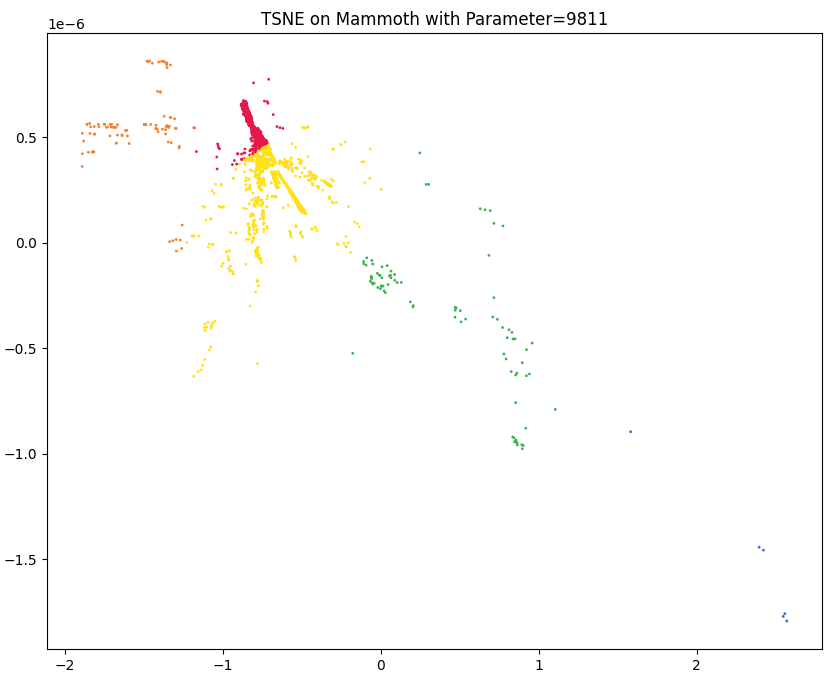
\includegraphics[width=\columnwidth]{images/KMEANS_5_TSNE_9811.png}
    	\caption{t-SNE $k=9811$}
        \label{fig:KMEANS_5_TSNE_9811}
    \end{subfigure}
     \caption[Clusters on low dim. 3D-Mammoth (local)]{Clusters on low dim. 3D-Mammoth (local), corresponding to Table \ref{tab:clu_mammoth}.}
    \label{fig:local_clu_mammoth}
\end{figure}

The Plan was to deploy not only $k$-Means but DBSCAN. This has to be canceled due to the misfortune of the application on the COIL-20 dataset (more details in Subsection \ref{subsec:clu_on_coil}) and due to the continuity of this dataset. Application of DBSCAN would most likely result in either a clustering where every point is a noise point or associated with a single cluster which is not what we intend to do.

\newpage

\section{Transformed 3D-Mammoth}

This section will deal with the transformed 3D-Mammoth dataset and is divided into subsections that one can also find in Section \ref{sec:exp.prod}.

\subsection{Distance Preservation}

Figure \ref{fig:DIST_transMammoth_all_B_and_A} shows us a comparison between 3D-Mammoth in lighter colors and transformed 3D-Mammoth in darker colors according to the distance preservation capabilities. Some exact values are displayed in Table \ref{tab:best_worst_dist_transMammoth}. The first thing we observe is that MDS's Frobenius norm dropped from $249$ to $248$ which explains why the light MDS graph cannot be seen in the plot as it is overlapping with the dark one. This means that the continuity property has no impact on the results of MDS. However, the continuity property has a significant impact on LLE and t-SNE. Until $p=666$ LLE performs worse on this dataset but then significantly better until it reaches a plateau at around $p\leq 1150$. Note that we did not deploy LLE on every parameter as we expected that it would reach a plateau because of the results we have seen from 3D-Mammoth in the previous section. It is likely that LLE would have a better Forbenius norm on a higher parameter setting, but this value would not be significantly better. On t-SNE, it seems that the overall shape of the graph remained the same but shifted up except for the values before $p= 570$ where it is performing significantly worse than t-SNE on the original 3D-Mammoth. According to these results, we suspect that LLE can perform better on non-continuous datasets. However, t-SNE seems to perform worse on these.

\begin{figure}[!]
	\centering
	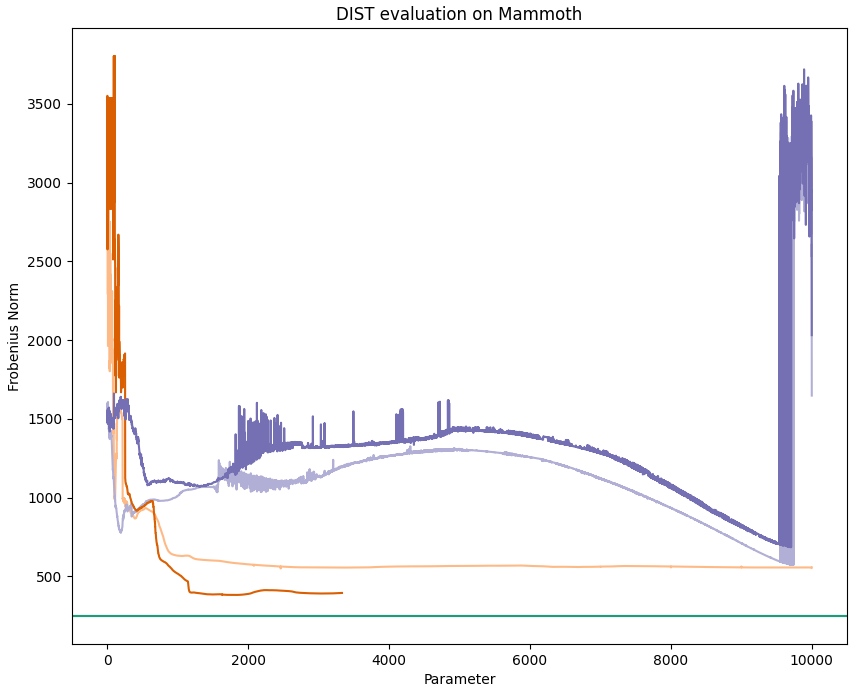
\includegraphics[width=1\columnwidth]{images/DIST_transMammoth_all_B_and_A.png}
	\caption[Transformed 3D-Mammoth Distance Preservation]{Plot showing the distance preservation capability of MDS, LLE, and t-SNE with different parameter settings. 3D-Mammoth in lighter and transformed 3D-Mammoth in darker colors. Note: MDS has no parameter.}
    \label{fig:DIST_transMammoth_all_B_and_A}
\end{figure}

\begin{table}[]
\centering
\begin{tabular}{|c|cl|cc|cc|}
\hline
 & \multicolumn{2}{c|}{{\color[HTML]{1b9e77} \textbf{MDS}}} & \multicolumn{2}{c|}{{\color[HTML]{d95f02} \textbf{LLE}}} & \multicolumn{2}{c|}{{\color[HTML]{7570B3} \textbf{t-SNE}}} \\ \hline
Rank & \multicolumn{2}{c|}{Frob. norm} & \multicolumn{1}{c|}{Param.} & Frob. norm & \multicolumn{1}{c|}{Param.} & Frob. norm \\ \hline
1 & \multicolumn{2}{c|}{\multirow{7}{*}{248}} & \multicolumn{1}{c|}{1788} & 381 & \multicolumn{1}{c|}{9706} & 684 \\ \cline{1-1} \cline{4-7} 
2 & \multicolumn{2}{c|}{} & \multicolumn{1}{c|}{1785} & 381 & \multicolumn{1}{c|}{9700} & 685 \\ \cline{1-1} \cline{4-7} 
3 & \multicolumn{2}{c|}{} & \multicolumn{1}{c|}{1793} & 381 & \multicolumn{1}{c|}{9677} & 685 \\ \cline{1-1} \cline{4-7} 
.. & \multicolumn{2}{c|}{} & \multicolumn{1}{c|}{..} & .. & \multicolumn{1}{c|}{..} & .. \\ \cline{1-1} \cline{4-7} 
9996 & \multicolumn{2}{c|}{} & \multicolumn{1}{c|}{105} & 3804 & \multicolumn{1}{c|}{9947} & 3657 \\ \cline{1-1} \cline{4-7} 
9997 & \multicolumn{2}{c|}{} & \multicolumn{1}{c|}{103} & 3804 & \multicolumn{1}{c|}{9948} & 3668 \\ \cline{1-1} \cline{4-7} 
9998 & \multicolumn{2}{c|}{} & \multicolumn{1}{c|}{98} & 3804 & \multicolumn{1}{c|}{9890} & 3719 \\ \hline
\end{tabular}
\caption[Transformed 3D-Mammoth Distance Preservation]{Best and worst results from transformed 3D-Mammoth concerning the distance preservation.}
\label{tab:best_worst_dist_transMammoth}
\end{table}

\subsection{Neighborhood Preservation}

Figure \ref{fig:1NN_transMammoth_all_B_and_A} shows us a comparison between 3D-Mammoth in lighter colors and transformed 3D-Mammoth in darker colors according to the neighborhood preservation capabilities. Some exact values are displayed in Table \ref{tab:best_worst_dist_transMammoth}. By looking at these results we see that the only thing that significantly changed is that the worst values for LLE shifted from around $k=9$ to around $k=159$. Every other trustworthiness value for every method did not change significantly. Therefore the graphs from 3D-Mammoth and the transformed 3D-Mammoth seem to fit very well onto one another. Because of these results, we state that the continuity property does not impact the neighborhood preservence of these methods. This can be explained by the fact that the transformation of the dataset did not have an impact on the distance of any nearest neighbor of a point. If, through the transformation, the nearest neighbor was pulled out of the neighborhood of one point it does not matter much because the second nearest neighbor is similarly close to it because of the continuity property.

\begin{figure}[!]
	\centering
	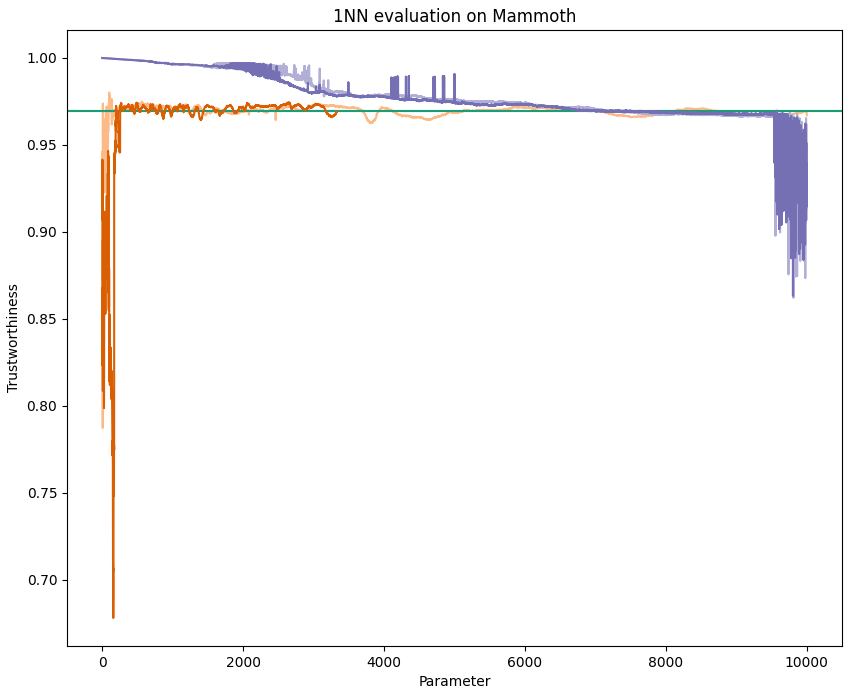
\includegraphics[width=1\columnwidth]{images/1NN_transMammoth_all_B_and_A.png}
	\caption[Transformed 3D-Mammoth Neighborhood Preservation]{Plot showing the neighborhood preservation capability of MDS, LLE, and t-SNE with different parameter settings. 3D-Mammoth in lighter and transformed 3D-Mammoth in darker colors. Note: MDS has no parameter.}
    \label{fig:1NN_transMammoth_all_B_and_A}
\end{figure}

\begin{table}[]
\centering
\begin{tabular}{|c|cl|cc|cc|}
\hline
 & \multicolumn{2}{c|}{{\color[HTML]{1B9E77} \textbf{MDS}}} & \multicolumn{2}{c|}{{\color[HTML]{D95F02} \textbf{LLE}}} & \multicolumn{2}{c|}{{\color[HTML]{7570B3} \textbf{t-SNE}}} \\ \hline
Rank & \multicolumn{2}{c|}{Trust.} & \multicolumn{1}{c|}{Param.} & Trust. & \multicolumn{1}{c|}{Param.} & Trust. \\ \hline
1 & \multicolumn{2}{c|}{} & \multicolumn{1}{c|}{2652} & 0.97 & \multicolumn{1}{c|}{2} & 1.00 \\ \cline{1-1} \cline{4-7} 
2 & \multicolumn{2}{c|}{} & \multicolumn{1}{c|}{2651} & 0.97 & \multicolumn{1}{c|}{3} & 1.00 \\ \cline{1-1} \cline{4-7} 
3 & \multicolumn{2}{c|}{} & \multicolumn{1}{c|}{2653} & 0.97 & \multicolumn{1}{c|}{4} & 1.00 \\ \cline{1-1} \cline{4-7} 
.. & \multicolumn{2}{c|}{} & \multicolumn{1}{c|}{..} & .. & \multicolumn{1}{c|}{..} & .. \\ \cline{1-1} \cline{4-7} 
1436 & \multicolumn{2}{c|}{} & \multicolumn{1}{c|}{158} & 0.70 & \multicolumn{1}{c|}{9776} & 0.88 \\ \cline{1-1} \cline{4-7} 
1437 & \multicolumn{2}{c|}{} & \multicolumn{1}{c|}{160} & 0.69 & \multicolumn{1}{c|}{9952} & 0.88 \\ \cline{1-1} \cline{4-7} 
1438 & \multicolumn{2}{c|}{\multirow{-7}{*}{0.97}} & \multicolumn{1}{c|}{159} & 0.68 & \multicolumn{1}{c|}{9803} & 0.86 \\ \hline
\end{tabular}
\caption[Transformed 3D-Mammoth Neighborhood Preservation]{Best and worst results from transformed 3D-Mammoth concerning the neighborhood preservation.}
\label{tab:best_worst_1nn_transMammoth}
\end{table}

\subsection{Visualization Quality} \label{subsec:visqual_transmamoth}

In this subsection, we will look at some comparisons of visualizations between the original and the transformed 3D-Mammoth dataset at some interesting parameter settings.

The first interesting comparison emerges by deploying LLE with $p=98$ between the original and the transformed 3D-Mammoth (Figure \ref{fig:mamm_vs_trans_98}). This shows us that if the dataset is continuous LLE can perform better with a lower parameter setting.

\begin{figure}[!]
     \centering
     \begin{subfigure}[t]{0.49\columnwidth}
    	\centering
    	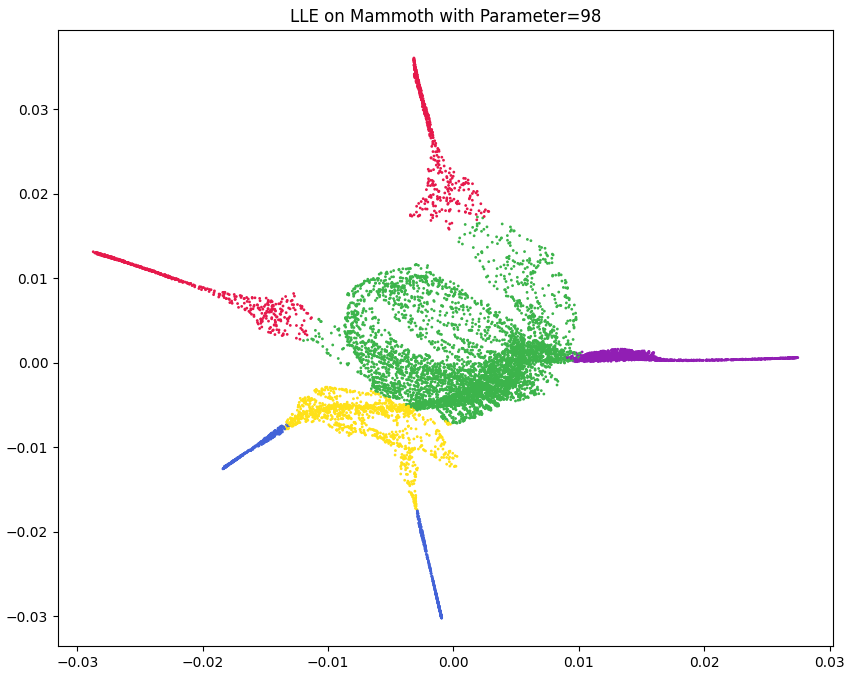
\includegraphics[width=\columnwidth]{images/LOW_Mammoth_lle_98.png}
    	\caption{3D-Mammoth with \\ $Forb.norm=1226$, $Trust.=0.98$}
        \label{fig:LOW_Mammoth_lle_98}
    \end{subfigure}
     \hfill
     \begin{subfigure}[t]{0.49\columnwidth}
    	\centering
    	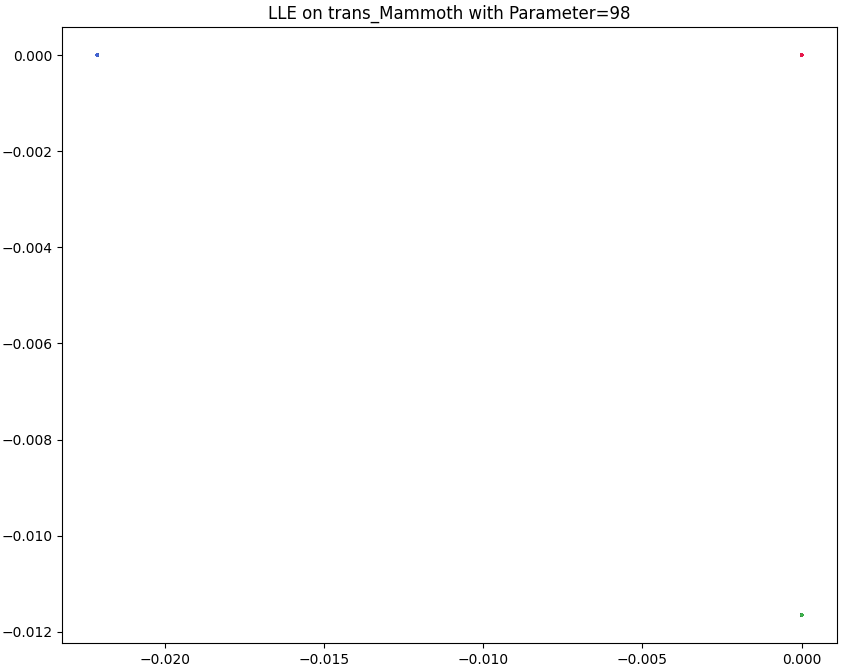
\includegraphics[width=\columnwidth]{images/LOW_trans_Mammoth_lle_98.png}
    	\caption{Transformed 3D-Mammoth  with \\ $Forb.norm=3804$, $Trust.=0.86$}
        \label{fig:LOW_trans_Mammoth_lle_98}
    \end{subfigure}
     \caption[3D-Mammoth vs. Transformed 3D-Mammoth Visualization]{Visualization of the embedding resulting from deploying LLE on both Mammoth datasets with $p=98$.}
    \label{fig:mamm_vs_trans_98}
\end{figure}

The next comparison in Figure \ref{fig:mamm_vs_trans_1788} shows two visualizations that have the same performance in neighborhood preservation. The visualization of the transformed 3D-Mammoth embedding is the best performing (distance preservation) parameter setting and the visualization of 3D-Mammoth embedding is also a very good performing one, compared to other results from this dataset. The interesting thing is that the non-continuous dataset can reach a lot better Frobenius norm scores (381 vs. 585) than the continuous one. We do not know how this comes.

\begin{figure}[!]
     \centering
     \begin{subfigure}[t]{0.49\columnwidth}
    	\centering
    	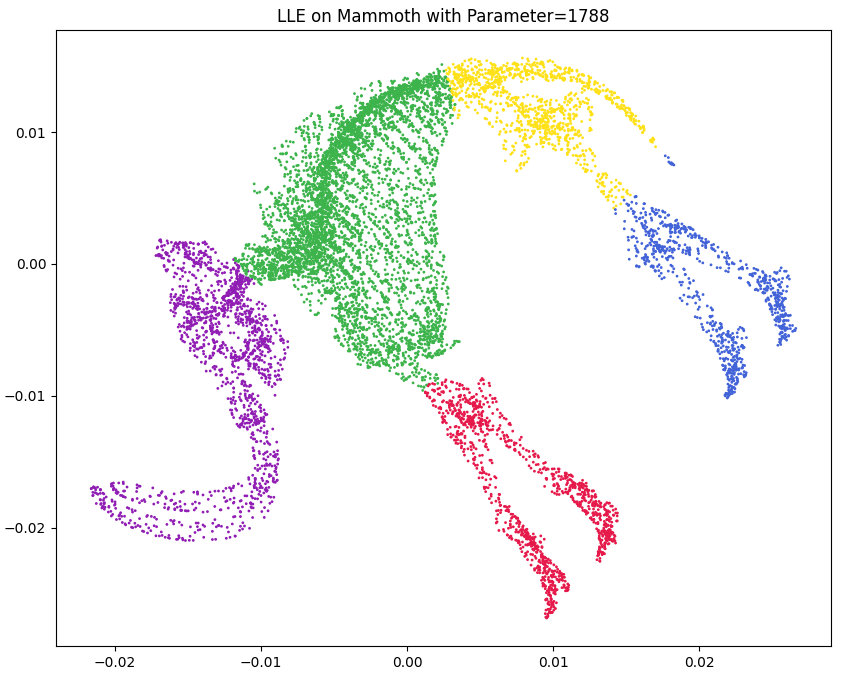
\includegraphics[width=\columnwidth]{images/LOW_Mammoth_lle_1788.png}
    	\caption{3D-Mammoth with \\ $Forb.norm=585$, $Trust.=0.97$}
        \label{fig:LOW_Mammoth_lle_1788}
    \end{subfigure}
     \hfill
     \begin{subfigure}[t]{0.49\columnwidth}
    	\centering
    	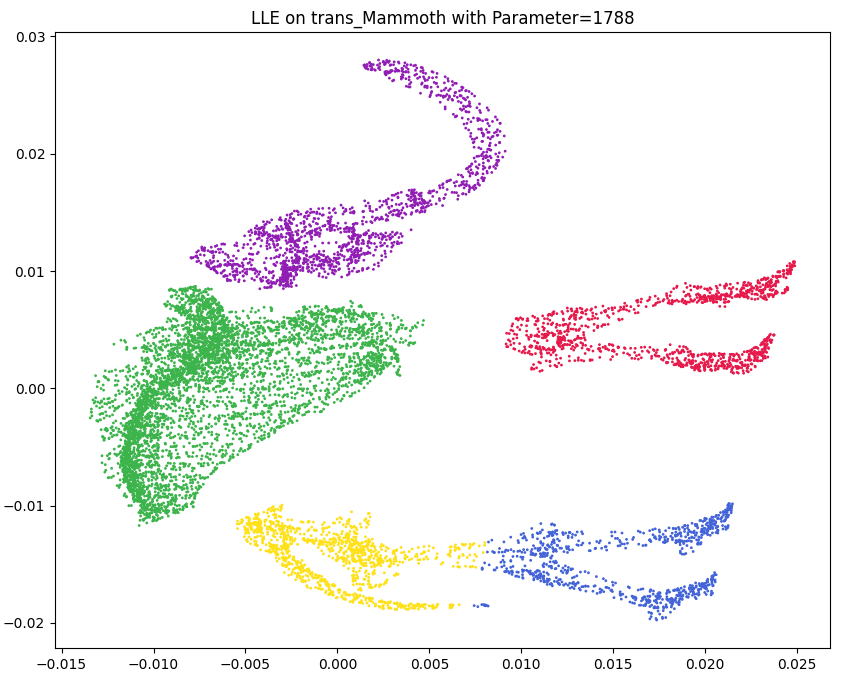
\includegraphics[width=\columnwidth]{images/LOW_trans_Mammoth_lle_1788.png}
    	\caption{Transformed 3D-Mammoth with \\ $Forb.norm=381$, $Trust.=0.97$}
        \label{fig:LOW_trans_Mammoth_lle_1788}
    \end{subfigure}
     \caption[3D-Mammoth vs. Transformed 3D-Mammoth Visualization]{Visualization of the embedding resulting from deploying LLE on both Mammoth datasets with $p=1788$.}
    \label{fig:mamm_vs_trans_1788}
\end{figure}

The third and last comparison (Figure \ref{fig:mamm_vs_trans_197}) is at $p=197$ in the t-SNE embeddings. We chose this comparison because this parameter setting was the best choice for t-SNE for the parameter settings. On 3D-Mammoth the performances after and before this parameter are getting worse. The interesting part is that by visual inspection, we can see that the structures/body parts themselves are preserved well which can be verified by the trustworthiness of both visualizations but the Frobenius norm, meaning the distance preserving (global structure) is a lot worse.

\begin{figure}[!]
     \centering
     \begin{subfigure}[t]{0.49\columnwidth}
    	\centering
    	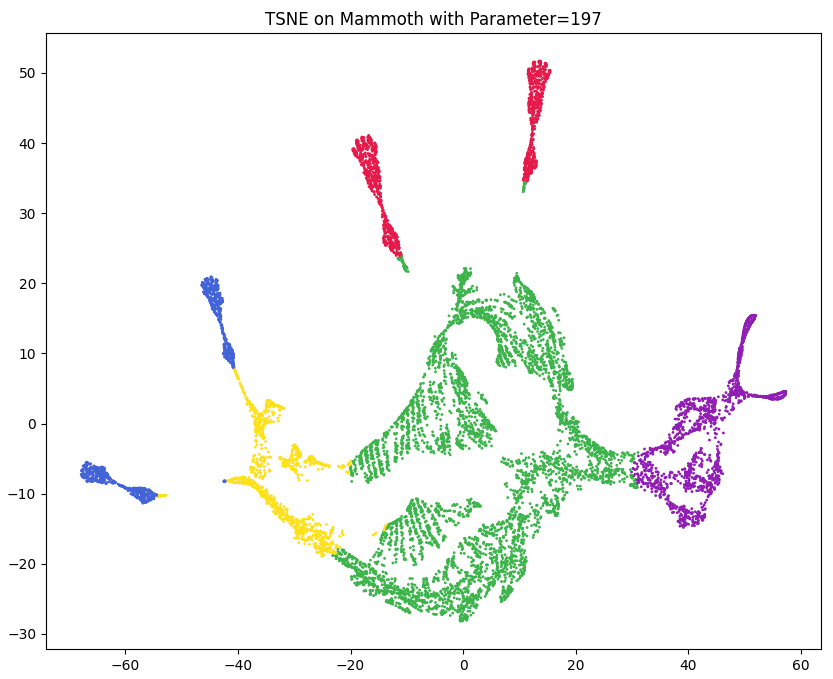
\includegraphics[width=\columnwidth]{images/LOW_Mammoth_tsne_197.png}
    	\caption{3D-Mammoth with \\ $Forb.norm=776$, $Trust.=0.97$}
        \label{fig:LOW_Mammoth_tsne_197}
    \end{subfigure}
     \hfill
     \begin{subfigure}[t]{0.49\columnwidth}
    	\centering
    	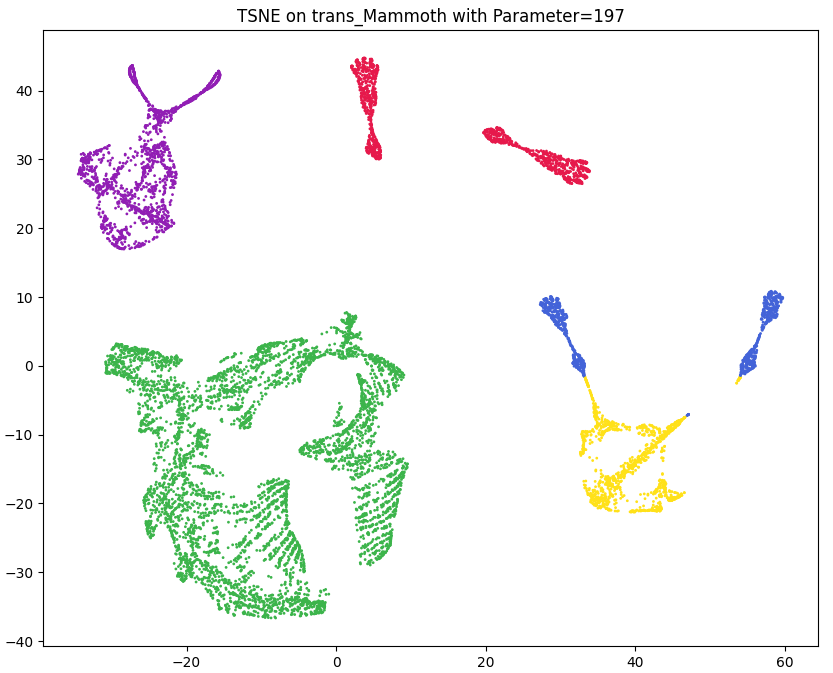
\includegraphics[width=\columnwidth]{images/LOW_trans_Mammoth_tsne_197.png}
    	\caption{Transformed 3D-Mammoth with \\ $Forb.norm=1599$, $Trust.=0.96$}
        \label{fig:LOW_trans_Mammoth_tsne_197}
    \end{subfigure}
     \caption[3D-Mammoth vs. Transformed 3D-Mammoth Visualization]{Visualization of the embedding resulting from deploying t-SNE on both Mammoth datasets with $p=197$.}
    \label{fig:mamm_vs_trans_197}
\end{figure}

\subsection{Clusterability on Embeddings} \label{subsec:clu_transmamm}

Similar to the subsection in 3D-Mammoth we again did run $k$-Means with different parameters to find the best one. The graph that arose from this parameter tuning step can be seen in Figure \ref{fig:SC_KMEANS_trans_MammothHighh}. If we compare this to the graph of the original 3D-Mammoth it is noticeable that the overall structure is pretty much the same. Just the best value is a little bit shifted so that the best value now yields from the parameter $k=2$ with $SC=0.47$. This result was somewhat unexpected. We instead expected the best silhouette score to be from $k=4$ because we transformed this dataset in a way where we get a natural clustering of 4. This result might be explained by the circumstance that the head is not very far from the rib cage whereas the rib cage is a lot more distant to the feet. 

\begin{figure}[!]
	\centering
	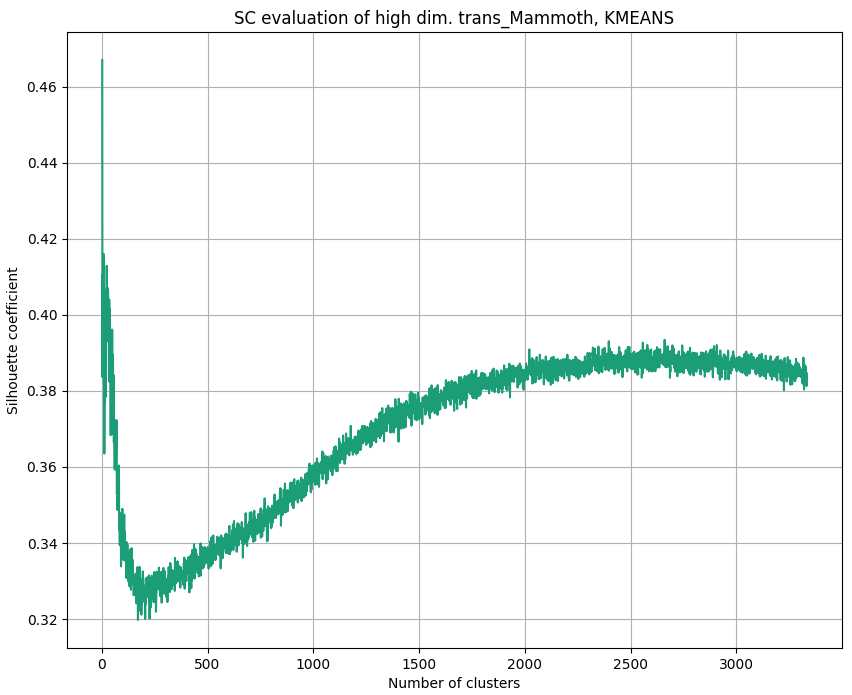
\includegraphics[width=0.85\columnwidth]{images/SC_KMEANS_trans_MammothHighh.png}
	\caption[Silhouette Scores for Transformed 3D-Mammoth]{Silhouette scores of high dimensional transformed 3D-Mammoth dataset after deploying $k$-Means with $2\leq k \leq 3333$.}
    \label{fig:SC_KMEANS_trans_MammothHighh}
\end{figure}

Figure \ref{fig:PLOT_trans_Mammoth_Kmeans2} shows how the best clustering according to the silhouette score on the transformed 3D-Mammoth datasets looks.

\begin{figure}[!]
	\centering
	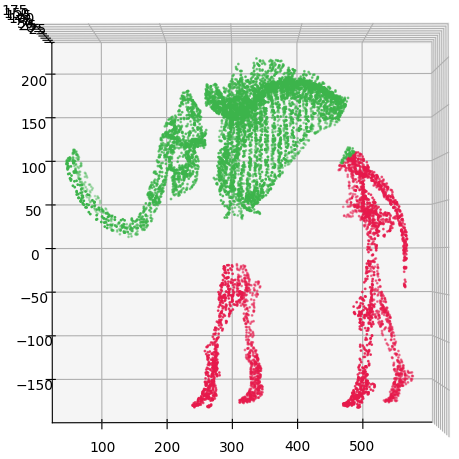
\includegraphics[width=0.5\columnwidth]{images/PLOT_trans_Mammoth_Kmeans2.png}
	\caption[Visualisation of Best Clustering for Transformed 3D-Mammoth]{Visualisation of the best $k$-Means clustering on transformed 3D-Mammoth with $k=2$, $SC=0.47$.}
    \label{fig:PLOT_trans_Mammoth_Kmeans2}
\end{figure}

Table \ref{tab:clu_trans_mammoth} shows the cluster evaluations on the low dimensional embeddings without the results of the worst-performing embeddings. We omit these because of the reason that these would likely have a good silhouette score but bad ARI and AMI scores as we have seen in \ref{subsec:clu_mamm}. We can again observe that good distance preservation does help a lot to get a good clustering. Both best local structure preserving runs are displayed in Figure \ref{fig:best_local_trans_mammoth_clu}. Those have an okay silhouette score but a bad and in the case of LLE with $p=2652$ even random clustering results according to the ARI and AMI scores. By looking at the visualizations it is noticeable that $2$-Means clustered the LLE embedding along the wrong axis. This happened because in this embedding the feet are a lot closer to the rib cage, nearly as close as the head is to the rib cage. Further, the results for t-SNE with $p=2$ emerged because half of all points are clustered at random and the other half was correct.

\begin{table}[]
\centering
\begin{tabular}{|c|c|c|c|c|c|}
\hline
\textbf{Type}            & \textbf{Method}                       & \textbf{Param.}          & \textbf{SC} & \textbf{ARI} & \textbf{AMI} \\ \hline
-                        & {\color[HTML]{1B9E77} \textbf{MDS}}   & {\color[HTML]{1B9E77} -} & 0.49        & 0.99         & 0.98         \\ \hline
                         & {\color[HTML]{D95F02} \textbf{LLE}}   & 1788                     & 0.47        & 0.89         & 0.83         \\ \cline{2-6} 
\multirow{-2}{*}{best global} & {\color[HTML]{7570B3} \textbf{t-SNE}} & 9706                     & 0.49        & 0.98         & 0.95         \\ \hline
                         & {\color[HTML]{D95F02} \textbf{LLE}}   & 2652                     & 0.37        & 0.01         & 0.00         \\ \cline{2-6} 
\multirow{-2}{*}{best local}  & {\color[HTML]{7570B3} \textbf{t-SNE}} & 2                        & 0.33        & 0.40         & 0.45         \\ \hline
\end{tabular}
\caption[Cluster Evaluation on Transformed 3D-Mammoth]{Cluster evaluation scores for low dimensional transformed 3D-Mammoth embeddings with $k=2$.}
\label{tab:clu_trans_mammoth}
\end{table}

\begin{figure}[!]
     \centering
     \begin{subfigure}[t]{0.49\columnwidth}
    	\centering
    	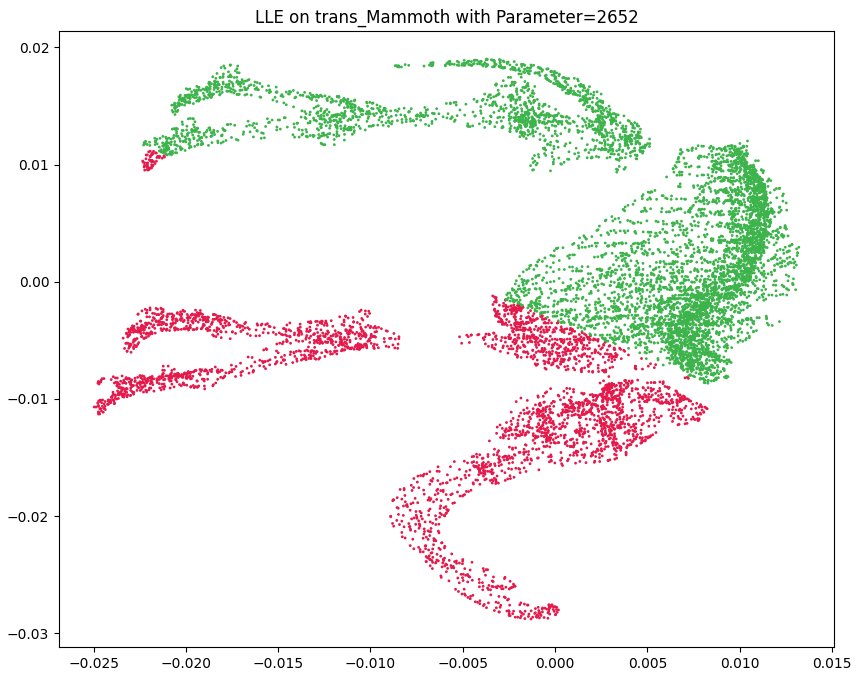
\includegraphics[width=\columnwidth]{images/LOW_trans_Mammoth_lle2652_Kmeans2.png}
    	\caption{LLE with $p=2652$}
        \label{fig:LOW_trans_Mammoth_lle2652_Kmeans2}
    \end{subfigure}
     \hfill
     \begin{subfigure}[t]{0.49\columnwidth}
    	\centering
    	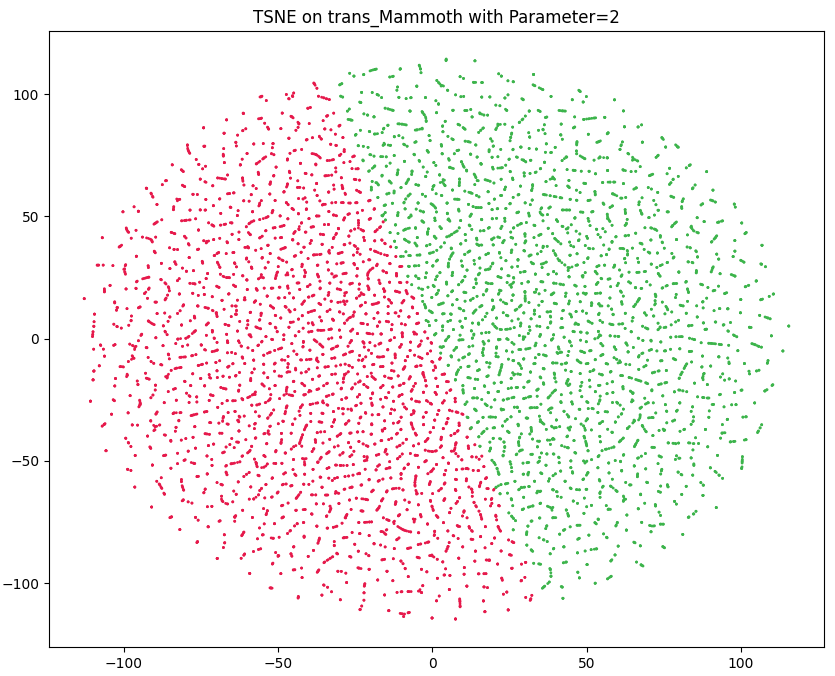
\includegraphics[width=\columnwidth]{images/LOW_trans_Mammoth_tsne2_Kmeans2.png}
    	\caption{t-SNE with $p=2$}
        \label{fig:LOW_trans_Mammoth_tsne2_Kmeans2}
    \end{subfigure}
     \caption[Best Local Transformed Mammoth Clustering]{Visualizations of the best local embeddings from transformed 3D-Mammoth datasets.}
    \label{fig:best_local_trans_mammoth_clu}
\end{figure}

Note that we did not deploy DBSCAN on this dataset because of similar reasons described in Subsection \ref{subsec:clu_mamm}.

\newpage

\section{COIL-20}

This section will deal with the COIL-20 dataset and is divided into subsections that one can also find in Section \ref{sec:exp.prod}. To get a feeling for the dataset and before diving deep into an analysis of the different methods it might be advantageous if we get an intuition of similarity in this specific dataset. This means that we will plot the heatmap of the pairwise distances in high dimensional space, translate the best and worst values back into the original images, and maybe verify if for example there are images of the same object but are classified as different or images of different objects that are classified as similar.

\begin{figure}[!]
	\centering
	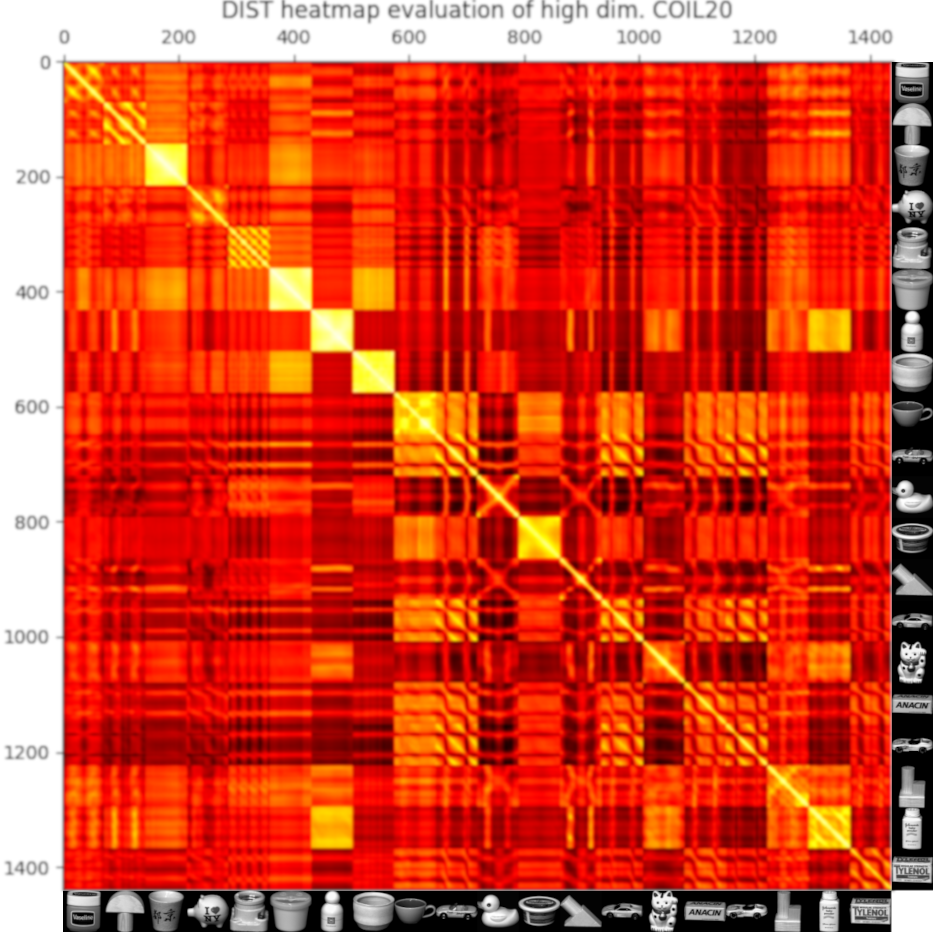
\includegraphics[width=1\columnwidth]{images/dist_heatmap_high_coil20.png}
	\caption[Heatmap of High COIL-20]{Heatmap of the high dimensional COIL-20 dataset. It is enriched with the corresponding images at some angle.}
    \label{fig:dist_heatmap_high_coil20}
\end{figure}

Figure \ref{fig:dist_heatmap_high_coil20} shows the high dimensional heatmap of COIL-20, meaning that we can see which images (objects at a specific angle) are similar to or different from one another. Every pixel represents the value of the pairwise distance between two images. The brighter the color the more similar and the darker the more different those images are. Every block of 72x72 pixels represents the comparison between objects at different angle settings. If a block is throughout very bright, e.g. the conditioner bottle (7) compared to itself, it means that the images of the objects are very similar to one another independent of the orientation of the object. An interesting note is that images of the same object do not necessarily have to be similar which can be seen in the block of the rubber duck (11) compared to itself. Also, there are interesting blocks such as (5,5) where a symmetric pattern is formed. This specific pattern means that if the compared image of the object is turned at an angle of 45° it looks different to the origin image but after turning the object again 45° (total of 90°) it looks very similar again. This is due to the fact that the object if viewed from above is symmetric in both ways, meaning that all 4 sides are identical but in the transition to one side the image has a view on a corner which is less similar to one of the side views. 

A similar example can be seen in Figure \ref{fig:dist_heatmap_high_coil20_wooden_bottle_anal} where there is again a pattern formed. The wooden piece illustrated at the top of the figure is similar to the powder bottle viewed from both sides but a lot less similar to the powder bottle viewed from the front or the back. Whereas the wooden piece illustrated at the bottom of the figure which is rotated by 180°, compared to the image, is almost equally similar to all orientations of the powder bottle. This might be because this image of the wooden object appears wider which is more similar to the front and back view of the powder bottle and has darker spots (shading) which are more similar to the dark writing of the front and back view of the bottle.

\begin{figure}[!]
	\centering
	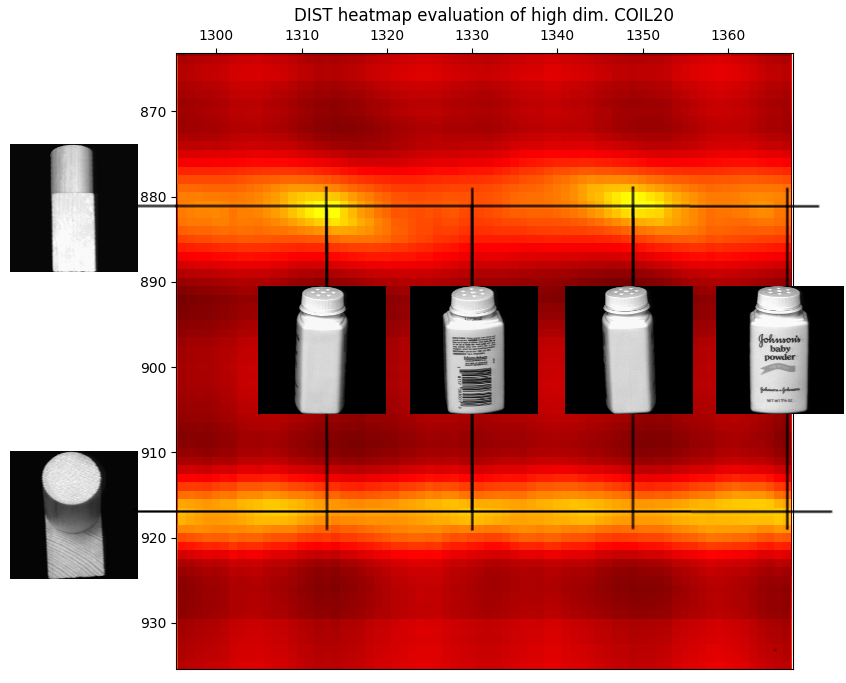
\includegraphics[width=1\columnwidth]{images/dist_heatmap_high_coil20_wooden_bottle_anal.png}
	\caption[Heatmap of Wooden Piece vs. Powder Bottle]{A 72x72 pixel block that emerged by zooming into the high dimensional COIL-20 heatmap. Enriched with images at specific angles. The line of pixels that are covered by the black line are the pairwise distances of images that are compared with the image the black line is starting from/passing through. Intersecting lines indicate the location of the value of the pairwise distance of those images.}
    \label{fig:dist_heatmap_high_coil20_wooden_bottle_anal}
\end{figure}

In Figure \ref{fig:most_similar_coil} the most similar objects are displayed. However, this insight is not very surprising as it is the same object, just turned at 5°. Therefore these images do just differ in nuances.

\begin{figure}[!]
     \centering
     \begin{subfigure}[t]{0.32\columnwidth}
    	\centering
    	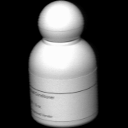
\includegraphics[width=\columnwidth]{images/coil-20-proc/obj7__49.png}
    	\caption{Deodorant bottle. \\ (obj7-49, $x,y=481$)}
        \label{fig:obj7__49}
    \end{subfigure}
     \hfill
     \begin{subfigure}[t]{0.32\columnwidth}
    	\centering
    	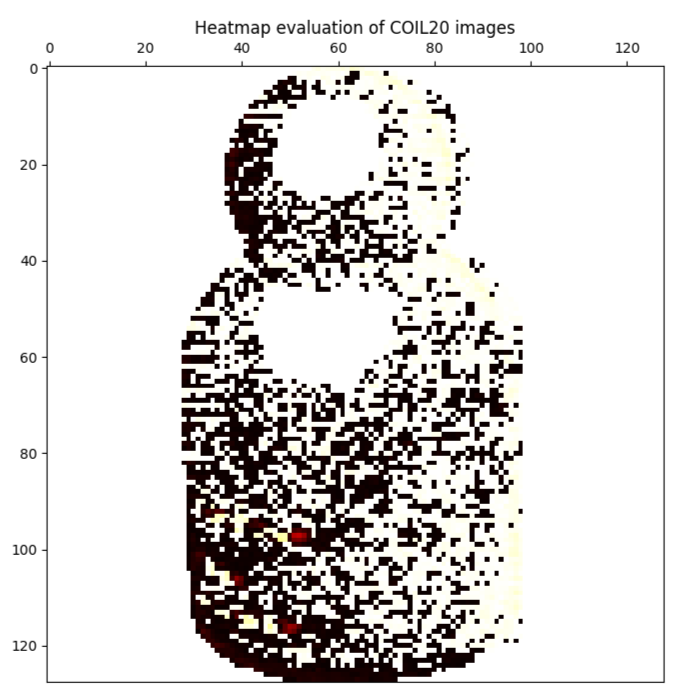
\includegraphics[width=\columnwidth]{images/heatmap_coil20_best.png}
    	\caption{Heatmap of the pixel difference.}
        \label{fig:heatmap_coil20_best}
    \end{subfigure}
     \hfill
     \begin{subfigure}[t]{0.32\columnwidth}
    	\centering
    	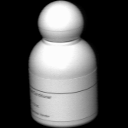
\includegraphics[width=\columnwidth]{images/coil-20-proc/obj7__50.png}
    	\caption{Deodorant bottle. \\ (obj7-50, $x,y=482$)}
        \label{fig:obj7__50}
    \end{subfigure}
     \caption[Most Similar COIL-20 Images]{The most similar images in the COIL-20 dataset. Note: The absolute difference is not as high as it seems. The color coding is not normalized with the maximal change possible in this dataset.}
    \label{fig:most_similar_coil}
\end{figure}

Figure \ref{fig:most_different_coil} shows the two images that are the most different (distant in high dimensional space) to one another. The image of the toy car represents an elongated object and the rubber duck on the other hand has a round form. The latter also covers a lot more space than the toy car and both just have different shadings. The difference can be seen visually in the heatmap. Note that the image background differs by 3 in greyscale, which might contribute a lot the the resulting difference. It might either be that in the processing of the images, something went wrong or that while taking the photos of the objects the researchers left a door/window open so that there was little light coming inside. The reason cannot be determined in retrospect due to the unavailability of the unprocessed versions of the images.

\begin{figure}[!]
     \centering
     \begin{subfigure}[t]{0.32\columnwidth}
    	\centering
    	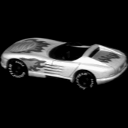
\includegraphics[width=\columnwidth]{images/coil-20-proc/obj17__4.png}
    	\caption{Toy car. \\ (obj17-4, $x,y=1156$)}
        \label{fig:obj17__4}
    \end{subfigure}
     \hfill
     \begin{subfigure}[t]{0.32\columnwidth}
    	\centering
    	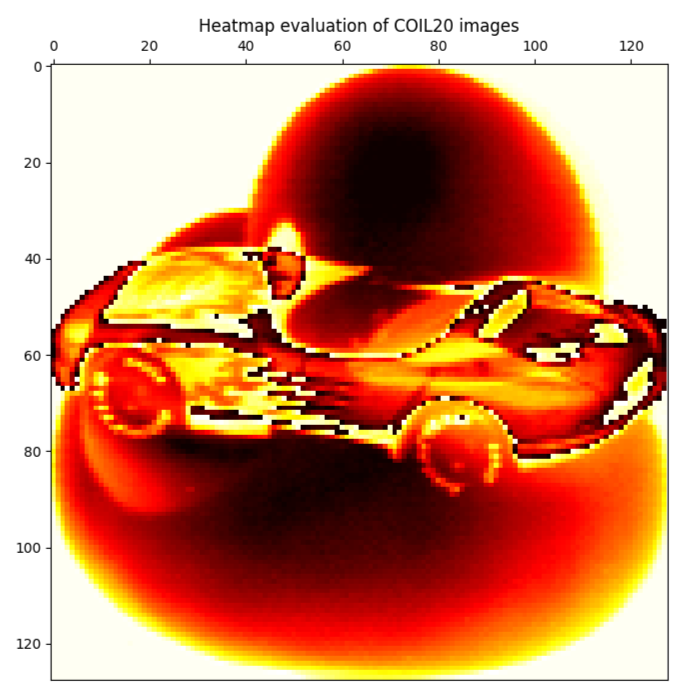
\includegraphics[width=\columnwidth]{images/heatmap_coil20_worst.png}
    	\caption{Heatmap of the pixel difference.}
        \label{fig:heatmap_coil20_worst}
    \end{subfigure}
     \hfill
     \begin{subfigure}[t]{0.32\columnwidth}
    	\centering
    	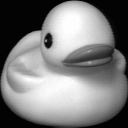
\includegraphics[width=\columnwidth]{images/coil-20-proc/obj11__49.png}
    	\caption{Rubber duck. \\ (obj11-49, $x,y=769$}
        \label{fig:obj11__49}
    \end{subfigure}
     \caption[Most Different COIL-20 Images]{The most different images in the COIL-20 dataset.}
    \label{fig:most_different_coil}
\end{figure}

Figure \ref{fig:first_most_different_coil} shows two images of the same object that are most different. Although it is the same object, one can see that these images are quite different. Mainly because of the different shadings (lighting on the obj) and the coverage of the space resulting from a non-symmetric property of the object.

\begin{figure}[!]
     \centering
     \begin{subfigure}[t]{0.32\columnwidth}
    	\centering
    	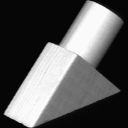
\includegraphics[width=\columnwidth]{images/coil-20-proc/obj13__27.png}
    	\caption{Wooden piece. \\ (obj13-27, $x,y=891$)}
        \label{fig:obj13__27}
    \end{subfigure}
     \hfill
     \begin{subfigure}[t]{0.32\columnwidth}
    	\centering
    	\includegraphics[width=\columnwidth]{images/heatmap_coil20_same.png}
    	\caption{Heatmap of the pixel difference.}
        \label{fig:heatmap_coil20_same}
    \end{subfigure}
     \hfill
     \begin{subfigure}[t]{0.32\columnwidth}
    	\centering
    	\includegraphics[width=\columnwidth]{images/coil-20-proc/obj13__12.png}
    	\caption{Wooden piece. \\ (obj13-12, $x,y=876$}
        \label{fig:obj13__12}
    \end{subfigure}
     \caption[Most Different of Same Object COIL-20 Images]{The most different images of the same object in the COIL-20 dataset.}
    \label{fig:first_most_different_coil}
\end{figure}

Lastly \ref{fig:first_most_different_coil} depict the most similar images of different objects. The overall shape and coverage of the space are very similar. Additionally, the shading contributes a lot to the similarity, especially on the bottom side of the objects. If the powder bottle is turned by 180° the similarity is comparably high because the powder bottle looks the same on the other side (is symmetric). 

\begin{figure}[!]
     \centering
     \begin{subfigure}[t]{0.32\columnwidth}
    	\centering
    	\includegraphics[width=\columnwidth]{images/coil-20-proc/obj13__17.png}
    	\caption{Wooden piece. \\ (obj13-17, $x,y=881$)}
        \label{fig:obj13__17}
    \end{subfigure}
     \hfill
     \begin{subfigure}[t]{0.32\columnwidth}
    	\centering
    	\includegraphics[width=\columnwidth]{images/heatmap_coil20_diff.png}
    	\caption{Heatmap of the pixel difference.}
        \label{fig:heatmap_coil20_diff}
    \end{subfigure}
     \hfill
     \begin{subfigure}[t]{0.32\columnwidth}
    	\centering
    	\includegraphics[width=\columnwidth]{images/coil-20-proc/obj19__53.png}
    	\caption{Powder bottle. \\ (obj19-53, $x,y=1349$)}
        \label{fig:obj19__53}
    \end{subfigure}
     \caption[Most Similar of Different Objects COIL-20 Images]{The most similar images of different objects in the COIL-20 dataset.}
    \label{fig:first_most_similar_coil}
\end{figure}

\subsection{Distance Preservation} \label{subsec:dist_coil}

By looking at Figure \ref{fig:dist_all_coil20_plot} and the corresponding Table \ref{tab:best_worst_dist_coil} MDS performs very well compared to the other methods considering that it does not need a parameter. But this is intuitive because the method itself optimizes for what we are evaluating in this evaluation. Namely the pairwise distance preservation. What is counter-intuitive is that despite this advantage of MDS, t-SNE on average exceeds the performance of MDS at around $p=900$ and significantly gets better until it reaches its unstable state at around $p\geq 1380$. We will elaborate on this in Section \ref{sec:rec_phen}. At low parameters, there is a specific parameter setting range ($15\leq p\leq 45$) where t-SNE performs very well. Looking at LLE's graph we see that it performs weakly in a low parameter setting but steadily gets better until it reaches more or less a plateau. What stands out is that LLE has some kinks where the performance is significantly worse than on adjacent parameter settings. We will elaborate on this in Section \ref{sec:rec_phen}. 

\begin{figure}[!]
	\centering
	\includegraphics[width=1\columnwidth]{images/dist_all_coil20_plot.png}
    \caption[COIL-20 Distance Preservation]{Plot showing the distance preservation capability of MDS, LLE, and t-SNE with different parameter settings. Note: MDS has no parameter.}
    \label{fig:dist_all_coil20_plot}
\end{figure}

\begin{table}[]
\centering
\begin{tabular}{|c|cl|cc|cc|}
\hline
 & \multicolumn{2}{c|}{{\color[HTML]{1b9e77} \textbf{MDS}}} & \multicolumn{2}{c|}{{\color[HTML]{d95f02} \textbf{LLE}}} & \multicolumn{2}{c|}{{\color[HTML]{7570B3} \textbf{t-SNE}}} \\ \hline
Rank & \multicolumn{2}{c|}{Frob. norm} & \multicolumn{1}{c|}{Param.} & Frob. norm & \multicolumn{1}{c|}{Param.} & Frob. norm \\ \hline
1 & \multicolumn{2}{c|}{\multirow{7}{*}{268}} & \multicolumn{1}{c|}{1229} & 303 & \multicolumn{1}{c|}{1403} & 244 \\ \cline{1-1} \cline{4-7} 
2 & \multicolumn{2}{c|}{} & \multicolumn{1}{c|}{1230} & 303 & \multicolumn{1}{c|}{1402} & 244 \\ \cline{1-1} \cline{4-7} 
3 & \multicolumn{2}{c|}{} & \multicolumn{1}{c|}{1231} & 303 & \multicolumn{1}{c|}{1399} & 244 \\ \cline{1-1} \cline{4-7} 
.. & \multicolumn{2}{c|}{} & \multicolumn{1}{c|}{..} & .. & \multicolumn{1}{c|}{..} & .. \\ \cline{1-1} \cline{4-7} 
1436 & \multicolumn{2}{c|}{} & \multicolumn{1}{c|}{19} & 787 & \multicolumn{1}{c|}{1388} & 848 \\ \cline{1-1} \cline{4-7} 
1437 & \multicolumn{2}{c|}{} & \multicolumn{1}{c|}{2} & 809 & \multicolumn{1}{c|}{1381} & 860 \\ \cline{1-1} \cline{4-7} 
1438 & \multicolumn{2}{c|}{} & \multicolumn{1}{c|}{3} & 821 & \multicolumn{1}{c|}{1390} & 868 \\ \hline
\end{tabular}
\caption[COIL-20 Distance Preservation]{Best and worst results from COIL-20 concerning the distance preservation.}
\label{tab:best_worst_dist_coil}
\end{table}

\subsection{Neighborhood Preservation}

The results of the evaluation of neighborhood preservation can be seen in Figure \ref{fig:1nn_all_coil20_plot} and in Table \ref{tab:best_worst_1nn_coil}. One can see that t-SNE overall has the best performance over most of the parameters but breaks in at very high parameter settings ($p \geq 1310$). MDS performs second best and LLE performs significantly worse than MDS across all parameter settings. This is very interesting because LLE is considered a local method and despite this fact, it does not perform better than MDS. LLE also performs weaker the lower the neighborhood size is but is very stable throughout moderate and high parameter settings.

\begin{figure}[!]
	\centering
	\includegraphics[width=1\columnwidth]{images/1nn_all_coil20_plot.png}
	\caption[COIL-20 Neighborhood Preservation]{Plot showing the neighborhood preservation capability of MDS, LLE, and t-SNE with different parameter settings. Note: MDS has no parameter.}
    \label{fig:1nn_all_coil20_plot}
\end{figure}

\begin{table}[]
\centering
\begin{tabular}{|c|cl|cc|cc|}
\hline
 & \multicolumn{2}{c|}{{\color[HTML]{1B9E77} \textbf{MDS}}} & \multicolumn{2}{c|}{{\color[HTML]{D95F02} \textbf{LLE}}} & \multicolumn{2}{c|}{{\color[HTML]{7570B3} \textbf{t-SNE}}} \\ \hline
Rank & \multicolumn{2}{c|}{Trust.} & \multicolumn{1}{c|}{Param.} & Trust. & \multicolumn{1}{c|}{Param.} & Trust. \\ \hline
1 & \multicolumn{2}{c|}{} & \multicolumn{1}{c|}{835} & 0.969 & \multicolumn{1}{c|}{2} & 1.000 \\ \cline{1-1} \cline{4-7} 
2 & \multicolumn{2}{c|}{} & \multicolumn{1}{c|}{986} & 0.969 & \multicolumn{1}{c|}{3} & 1.000 \\ \cline{1-1} \cline{4-7} 
3 & \multicolumn{2}{c|}{} & \multicolumn{1}{c|}{993} & 0.968 & \multicolumn{1}{c|}{4} & 1.000 \\ \cline{1-1} \cline{4-7} 
.. & \multicolumn{2}{c|}{} & \multicolumn{1}{c|}{..} & .. & \multicolumn{1}{c|}{..} & .. \\ \cline{1-1} \cline{4-7} 
1436 & \multicolumn{2}{c|}{} & \multicolumn{1}{c|}{4} & 0.837 & \multicolumn{1}{c|}{1418} & 0.887 \\ \cline{1-1} \cline{4-7} 
1437 & \multicolumn{2}{c|}{} & \multicolumn{1}{c|}{3} & 0.824 & \multicolumn{1}{c|}{1416} & 0.881 \\ \cline{1-1} \cline{4-7} 
1438 & \multicolumn{2}{c|}{\multirow{-7}{*}{0.976}} & \multicolumn{1}{c|}{2} & 0.722 & \multicolumn{1}{c|}{1417} & 0.872 \\ \hline
\end{tabular}
\caption[COIL-20 Neighborhood Preservation]{Best and worst results from COIL-20 concerning the neighborhood preservation.}
\label{tab:best_worst_1nn_coil}
\end{table}

\subsection{Visualization Quality}

The fact that COIL-20 is a high dimesnional dataset consisting of images leads to low-dimensional embeddings that if plotted do not convey much meaning. Therefore we will showcase in Figure \ref{fig:low_coil_plots} how some example embeddings could look like but we will not go into detail on them. 

\begin{figure}[!]
     \centering
     \begin{subfigure}[t]{0.55\columnwidth}
    	\centering
    	\includegraphics[width=\columnwidth]{images/plot_mds_coil20.png}
    	\caption{MDS, $Forb.norm=267$, $Trust.=0.98$}
        \label{fig:plot_mds_coil20}
    \end{subfigure}
     \hfill
     \begin{subfigure}[t]{0.55\columnwidth}
    	\centering
    	\includegraphics[width=\columnwidth]{images/plot_lle_coil20_3.png}
    	\caption{LLE with $p=3$, $Forb.norm=821$, $Trust.=0.82$}
        \label{fig:plot_lle_coil20_3}
    \end{subfigure}
     \hfill
     \begin{subfigure}[t]{0.55\columnwidth}
    	\centering
    	\includegraphics[width=\columnwidth]{images/plot_tsne_coil20_1390.png}
    	\caption{t-SNE with $p=1390$, $Forb.norm=868$, $Trust.=0.95$}
        \label{fig:plot_tsne_coil20_1390}
    \end{subfigure}
     \caption[Low Dimensional COIL-20 Plots]{Plot of some specific embeddings that emerged by reducing the dimensionality of COIL-20.}
    \label{fig:low_coil_plots}
\end{figure}

Instead, we will take a closer look at the heatmaps that arise by either calculating the pairwise distances in a low-dimensional embedding or by subtracting these from the pairwise distances from the high-dimensional space. The latter heatmap can be seen in Figure \ref{fig:dist_heatmap_high_coil20} that we introduced earlier in this section. On the heatmaps (pairwise distance matrix) that are processed beforehand, meaning that they were subtracted from the high dimensional heatmaps one can see which pairwise distances could be preserved and which not. Whereas the semantics of the low-dimensional heatmaps are different. These only display how distant the images/datapoints are embedded from each other.

In Figure \ref{fig:heat_best} the best distance preservations for all methods are displayed. By visually inspecting those one can see that t-SNE overall performs best and LLE worst which is reflected by the results in Subsection \ref{subsec:dist_coil}. It is also obvious that in all three heatmaps, the manifold learning methods had difficulties with the same images, as far as we can tell visually, which can be seen in similar patterns throughout the heatmaps. The common characteristic of those images is that they are very distant in high dimensional space which means that it is more difficult for those methods to preserve the distance of distant datapoints than similar datapoints. This can be explained by the crowding problem.

\begin{figure}[!]
     \centering
     \begin{subfigure}[t]{0.32\columnwidth}
    	\centering
    	\includegraphics[width=\columnwidth]{images/dist_heatmap_mds_coil20_None.png}
    	\caption{MDS.}
        \label{fig:dist_heatmap_mds_coil20_None}
    \end{subfigure}
     \hfill
     \begin{subfigure}[t]{0.32\columnwidth}
    	\centering
    	\includegraphics[width=\columnwidth]{images/dist_heatmap_lle_coil20_1-3best.png}
    	\caption{LLE with \\ $p=1229,1230,1231$}
        \label{fig:dist_heatmap_lle_coil20_1-3best}
    \end{subfigure}
     \hfill
     \begin{subfigure}[t]{0.32\columnwidth}
    	\centering
    	\includegraphics[width=\columnwidth]{images/dist_heatmap_tsne_coil20_1-3best.png}
    	\caption{t-SNE with \\ $p=1403,1402,1399$}
        \label{fig:dist_heatmap_tsne_coil20_1-3best}
    \end{subfigure}
     \caption[Heatmaps of Best Distance Preservations]{Heatmaps of the best distance preservation tries, already subtracted to the high-dimensional heatmap.}
    \label{fig:heat_best}
\end{figure}

Looking at the worst embeddings of LLE (Figure \ref{fig:heat_worst_coil_lle} we observe that all three embeddings have very different pairwise distances. What is outstanding is that every embedding chose different images to optimize the LLE cost function and completely ignored the rest which is embedded in the same spot (collapsing). Interestingly LLE somehow can detect coherent regions, in our case objects. We could not observe a pattern in which images or clusters of images (objects) were preferably embedded well.

\begin{figure}[!]
     \centering
     \begin{subfigure}[t]{0.49\columnwidth}
    	\centering
    	\includegraphics[width=\columnwidth]{images/dist_heatmap_lle_coil20_1worst_beforediff.png}
    	\caption{1. worst LLE embedding with $p=3$}
        \label{fig:dist_heatmap_lle_coil20_1worst_beforediff}
    \end{subfigure}
     \hfill
     \begin{subfigure}[t]{0.49\columnwidth}
    	\centering
    	\includegraphics[width=\columnwidth]{images/dist_heatmap_lle_coil20_1worst.png}
    	\caption{1. worst LLE embedding with $p=3$}
        \label{fig:dist_heatmap_lle_coil20_1worst}
    \end{subfigure}
     \hfill
     \begin{subfigure}[t]{0.49\columnwidth}
    	\centering
    	\includegraphics[width=\columnwidth]{images/dist_heatmap_lle_coil20_2worst_beforediff.png}
    	\caption{2. worst LLE embedding with $p=2$}
        \label{fig:dist_heatmap_lle_coil20_2worst_beforediff}
    \end{subfigure}
     \hfill
     \begin{subfigure}[t]{0.49\columnwidth}
    	\centering
    	\includegraphics[width=\columnwidth]{images/dist_heatmap_lle_coil20_2worst.png}
    	\caption{2. worst LLE embedding with $p=2$}
        \label{fig:dist_heatmap_lle_coil20_2worst}
    \end{subfigure}
     \hfill
     \begin{subfigure}[t]{0.49\columnwidth}
    	\centering
    	\includegraphics[width=\columnwidth]{images/dist_heatmap_lle_coil20_3worst_beforediff.png}
    	\caption{3. worst LLE embedding with $p=19$}
        \label{fig:dist_heatmap_lle_coil20_3worst_beforediff}
    \end{subfigure}
     \hfill
     \begin{subfigure}[t]{0.49\columnwidth}
    	\centering
    	\includegraphics[width=\columnwidth]{images/dist_heatmap_lle_coil20_3worst.png}
    	\caption{3. worst LLE embedding with $p=19$}
        \label{fig:dist_heatmap_lle_coil20_3worst}
    \end{subfigure}
     \caption[Heatmaps of Worst LLE Distance Preservations]{Heatmaps of the worst distance preservation tries. The left side depicts the heatmaps before subtraction and the right side after.}
    \label{fig:heat_worst_coil_lle}
\end{figure}

The worst distance preservation embeddings of t-SNE are quite different than the ones from LLE (Figure \ref{fig:heat_worst_coil_tsne}). T-SNE does not favor any datapoints, instead, although collapsing on some points, it mostly tries to embed points with some distance.

\begin{figure}[!]
     \centering
     \begin{subfigure}[t]{0.49\columnwidth}
    	\centering
    	\includegraphics[width=\columnwidth]{images/dist_heatmap_tsne_coil20_1-3wors_beforediff.png}
    	\caption{Worst t-SNE embeddings \\ with $p=1390,1381,1388$}
        \label{fig:dist_heatmap_tsne_coil20_1-3wors_beforediff}
    \end{subfigure}
     \hfill
     \begin{subfigure}[t]{0.49\columnwidth}
    	\centering
    	\includegraphics[width=\columnwidth]{images/dist_heatmap_tsne_coil20_1-3worst.png}
    	\caption{Worst t-SNE embeddings \\ with $p=1390,1381,1388$}
        \label{fig:dist_heatmap_tsne_coil20_1-3worst}
    \end{subfigure}
     \caption[Heatmaps of Worst t-SNE Distance Preservations]{Heatmaps of the worst distance preservation tries. The left side depicts the heatmaps before subtraction and the right side after.}
    \label{fig:heat_worst_coil_tsne}
\end{figure}

\subsection{Clusterability on Embeddings} \label{subsec:clu_on_coil}

To evaluate the clusterability of COIL-20 embeddings we chose the number of clusters in two ways. One way was to use already existing clusters from the dataset and the other way was to calculate them. By using the first way we assigned images of one object to one cluster resulting in a total of 20 clusters (number of objects) and assigned images of one angle to one cluster resulting in a total of 72 clusters (number of angles). Corresponding to these number of clusters we also deployed $k$-Means with $k\in\{20,72\}$. Luckily $k=72$ already represents the best possible clustering according to the silhouette score (Figure \ref{fig:SC_KMEANS_COIL20_high}. The results, meaning the silhouette, ARI, and AMI scores are displayed in Table \ref{tab:clu_coil}. Note that we did not evaluate the clusterability of the bad-performing runs of the manifold learning methods because of the reasons mentioned in \ref{subsec:clu_mamm}.

At first, it was not in our plan to calculate our own clustering but by looking into the silhouette scores of the clustering that naturally emerge from the dataset we had to realize that these are bad clusterings. The silhouette score from one cluster per object ($k=20$) yielded $sc=0.16$. By calculating our own 20 clusters we got a significantly better clustering with $sc=0.21$. The same applies to the cluster per angle ($k=72$) approach where this yielded $sc=-0.07$ and by calculating our own 72 clusters we got $sc=0.28$. To humble ourselves we have to admit that the latter was quite predictable because it is very unlikely that assigning every angle option to one cluster will form a good clustering.

\begin{figure}[!]
	\centering
	\includegraphics[width=0.85\columnwidth]{images/SC_KMEANS_COIL20_high.png}
	\caption[Silhouette Scores for COIL-20]{Silhouette scores of high dimensional COIL-22 dataset after deploying $k$-Means for all possible $k$.}
    \label{fig:SC_KMEANS_COIL20_high}
\end{figure}

\begin{table}[]
\centering
\begin{tabular}{cc|c|c|cc|cc|}
\cline{3-8}
 &  & \textbf{Type} & - & \multicolumn{2}{c|}{best global} & \multicolumn{2}{c|}{best local} \\ \cline{3-8} 
 &  & \textbf{Method} & {\color[HTML]{1B9E77} \textbf{MDS}} & \multicolumn{1}{c|}{{\color[HTML]{D95F02} \textbf{LLE}}} & {\color[HTML]{7570B3} \textbf{t-SNE}} & \multicolumn{1}{c|}{{\color[HTML]{D95F02} \textbf{LLE}}} & {\color[HTML]{7570B3} \textbf{t-SNE}} \\ \cline{3-8} 
 &  & \textbf{Param.} & {\color[HTML]{000000} -} & \multicolumn{1}{c|}{1229} & 1403 & \multicolumn{1}{c|}{835} & 2 \\ \hline
\multicolumn{1}{|c|}{} & low dim. & \textbf{SC} & 0.41 & \multicolumn{1}{c|}{0.45} & 0.49 & \multicolumn{1}{c|}{0.46} & 0.27 \\ \cline{2-8} 
\multicolumn{1}{|c|}{} &  & \textbf{ARI} & 0.55 & \multicolumn{1}{c|}{0.53} & 0.50 & \multicolumn{1}{c|}{0.50} & 0.38 \\ \cline{3-8} 
\multicolumn{1}{|c|}{} & \multirow{-2}{*}{orig.} & \textbf{AMI} & 0.73 & \multicolumn{1}{c|}{0.73} & 0.71 & \multicolumn{1}{c|}{0.70} & 0.65 \\ \cline{2-8} 
\multicolumn{1}{|c|}{} &  & \textbf{ARI} & 0.52 & \multicolumn{1}{c|}{0.51} & 0.50 & \multicolumn{1}{c|}{0.50} & 0.25 \\ \cline{3-8} 
\multicolumn{1}{|c|}{\multirow{-5}{*}{k=20}} & \multirow{-2}{*}{calc.} & \textbf{AMI} & 0.73 & \multicolumn{1}{c|}{0.72} & 0.70 & \multicolumn{1}{c|}{0.70} & 0.53 \\ \hline
\multicolumn{1}{|c|}{} & low dim. & \textbf{SC} & 0.41 & \multicolumn{1}{c|}{0.41} & 0.45 & \multicolumn{1}{c|}{0.41} & 0.37 \\ \cline{2-8} 
\multicolumn{1}{|c|}{} &  & \textbf{ARI} & -0.01 & \multicolumn{1}{c|}{-0.01} & -0.01 & \multicolumn{1}{c|}{-0.01} & -0.01 \\ \cline{3-8} 
\multicolumn{1}{|c|}{} & \multirow{-2}{*}{orig.} & \textbf{AMI} & -0.05 & \multicolumn{1}{c|}{-0.05} & -0.06 & \multicolumn{1}{c|}{-0.06} & -0.04 \\ \cline{2-8} 
\multicolumn{1}{|c|}{} &  & \textbf{ARI} & 0.62 & \multicolumn{1}{c|}{0.56} & 0.58 & \multicolumn{1}{c|}{0.59} & 0.35 \\ \cline{3-8} 
\multicolumn{1}{|c|}{\multirow{-5}{*}{k=72}} & \multirow{-2}{*}{calc.} & \textbf{AMI} & 0.72 & \multicolumn{1}{c|}{0.71} & 0.71 & \multicolumn{1}{c|}{0.72} & 0.66 \\ \hline
\end{tabular}
\caption[Cluster Evaluation on COIL-20]{Scores for low dimensional COIL-20 embeddings. While the configuration (k=20, orig.) means one cluster per object, (k=72, orig.) means one cluster per angle, (k=20, calc.) and (k=72, calc.) mean that the clustering was calculated with $k$-Means.}
\label{tab:clu_coil}
\end{table}

The results in Table \ref{tab:clu_coil} show us that for both $k$ the global structure preserved t-SNE embedding performs best in terms of silhouette score. The local structure preserved t-SNE embedding however scores worst on all possible scores meaning that an embedding that preserved the local structure well by t-SNE does not enable good clustering. Further, for both the original and calculated 20 cluster and 72 cluster settings, according to the ARI and AMI scores, MDS overall performs best but it is not significantly better than the results from t-SNE and LLE. The results for the original $k=72$ clustering verify that this clustering represents a random clustering.

\begin{figure}[!]
	\centering
	\includegraphics[width=0.85\columnwidth]{images/SC_DBSCAN_COIL20_high.png}
	\caption[DBSCAN on COIL-20]{Silhouette score resulting from deploying DBSCAN on COIL-20 with different parameter setting, displayed as a heatmap. Blue dots point on the two best results. Note: Clustering results where every point was marked as noise or results where every point was in a single cluster where mapped to the worst possible value -1.}
    \label{fig:SC_DBSCAN_COIL20_high}
\end{figure}

Figure \ref{fig:SC_DBSCAN_COIL20_high} shows our approach of deploying and parameter tuning DBSCAN on the high dimensional COIL-20 dataset with the expectation to yield two best $eps$ and $minPts$ parameters that we could use to deploy DBSCAN on the low dimensional embeddings. The heatmap is a grid that depicts the silhouette scores for 16 $eps$ x 15 $minPts$ values. By successively zooming into (calculating values in between) the two best results could be determined. Those were $eps=12340$, $minPts=1312$ with $SC=0.20$ and $eps=8920$, $minPts=2$ with $SC=0.19$. However, by further analyzing these results, we noticed that the best result was a clustering where one point was classified as noise and all others were classified into a single cluster. The second best result was a clustering where 2 points were classified into one cluster and every other point was classified into another cluster. These were not the results we expected. Because of this, we chose not to continue with this clustering algorithm. Another reason was that it is very hard, maybe not possible, to tune the parameters in high dimensional space and use them in the low dimensional embedding because of the parameter $eps$. This parameter cannot be reused because by reducing the dimensionality of a dataset the distances between points do also get less.

\newpage

\section{Recurring Phenomena} \label{sec:rec_phen}

In this section, we will elaborate on phenomena that often occured in our experiments regarding manifold learning methods.

\subsection{LLE's Unstableness}

In every graph of lle, whether it was the parameter tuning of the distance or the neighborhood preservation, we could observe the phenomena where at some parameter setting the embedding suddenly performed significantly worse or better than the adjacent parameter settings resulting in kinks. This phenomenon was less obvious in the results of the original and the transformed Mammoth because these had a lot more possible parameters and a higher range of possible values which led to a compressed graph, but they existed.
The unstableness of lle on those parameter settings is explained by the eigensolver method that sklearn uses.\footnotemark They use arpack (arnoldi iteration in shift-invert mode) to enhance the computation speed. This comes with the trade-off that the calculation might be disturbed. We could verify that with the standard dense matrix for eigenvalue decomposition. The values line up perfectly with the course of the graphs which can be seen in Figure \ref{fig:kinks_lle}. What this means is that these anomalies do not occur because of dataset specifics.
\footnotetext{\url{https://scikit-learn.org/stable/modules/generated/sklearn.manifold.LocallyLinearEmbedding.html}}

\begin{figure}[!]
     \centering
     \begin{subfigure}[t]{0.49\columnwidth}
    	\centering
    	\includegraphics[width=\columnwidth]{images/dist_dense_coil20.png}
    	\caption{Distance preservation}
        \label{fig:dist_dense_coil20}
    \end{subfigure}
     \hfill
     \begin{subfigure}[t]{0.49\columnwidth}
    	\centering
    	\includegraphics[width=\columnwidth]{images/1NN_dense_plot.png}
    	\caption{Neighborhood preservation}
        \label{fig:1NN_dense_plot}
    \end{subfigure}
     \caption[Kinks in LLE's Graphs]{Evaluation plots on COIL-20 showing LLE graphs with kinks. Black dots represent the results on those parameter settings where those anomalies occur. For these executions dense-LLE was used.}
    \label{fig:kinks_lle}
\end{figure}

\subsection{t-SNE's Unstableness}

On all distance evaluations where we deployed t-SNE on very high parameter settings, we could observe the phenomena where the Frobenius norm was oscillating extremely between the best and worst values. On all neighborhood preservation evaluations, this phenomenon did not occur to this extent but still, it was there. Because this happened in all of our evaluations we can exclude the effect of dataset specificities. To further exclude the influence of the non-deterministic behavior of t-SNE we deployed it with different initialization strategies. On the one hand with PCA initialization and on the other hand with random initializations, because these are the only strategies that sklearn supports.\footnotemark The results of these initalizations can be seen in Figure \ref{fig:osc_tsne}. We can clearly see that the initialization and therefore the non-deterministic property of t-SNE did not have any significant impact on this phenomenon. In our research, we could not find the exact reason for this anomaly. The only thing we can state is that this occurred in all our experiments which speaks for the fact that it is a peculiarity of t-SNE which has to be further investigated in future work.
\footnotetext{\url{https://scikit-learn.org/stable/modules/generated/sklearn.manifold.TSNE.html}}

\begin{figure}[!]
     \centering
     \begin{subfigure}[t]{0.49\columnwidth}
    	\centering
    	\includegraphics[width=\columnwidth]{images/dist_tsne_coil20_1375_1440_1.png}
    	\caption{PCA initialized t-SNE.}
        \label{fig:dist_tsne_coil20_1375_1440_1}
    \end{subfigure}
     \hfill
     \begin{subfigure}[t]{0.49\columnwidth}
    	\centering
    	\includegraphics[width=\columnwidth]{images/dist_tsne_coil20_1340_1440_1_random.png}
    	\caption{Random initialized t-SNE.}
        \label{fig:dist_tsne_coil20_1340_1440_1_random}
    \end{subfigure}
     \caption[Oscillation on t-SNE's Graphs]{Evaluation plots on COIL-20 showing t-SNE graphs with extreme oscillations.}
    \label{fig:osc_tsne}
\end{figure}

\newpage

\section{Derived Knowledge}

In this section, we will summarize the insight that we could derive from our experiments and give some useful tips for the successful deployment of the manifold learning methods we used.

\paragraph{Best Methods for Distance Preservation.}
The best method to use when it comes to optimizing the distance preservation of a low-dimensional embedding of a dataset is MDS. This is not surprising because MDS optimizes its loss function for this. However, in the case of the COIL-20 dataset t-SNE performed on some high-parameter settings better than MDS. LLE performed better than t-SNE on 3D-Mammoths but worse on COIL-20.

\paragraph{Best Methods for Neighborhood Preservation.}
The best method to use when it comes to optimizing the neighborhood preservation of a low-dimensional embedding of a dataset is t-SNE with low parameter settings. On 3D-Mammoth datasets LLE and MDS performed equally well and for COIL-20 MDS performed significantly better. These statements are rather unexpected because LLE is considered a local method that emphasizes the local structure preservence. MDS however which is a global method performs equally well, even better in the case of COIL-20.

\paragraph{Continuity property does not impact MDS, impacts LLE for the better, and t-TNE for the worse.}
By comparing the results for the original 3D-Mammoth and the transformed 3D-Mammoth it was noticeable that MDS performed the same one both. However, the performance, regarding the distance preservation of LLE, was impacted in a positive way where significantly better Forbenius norms were scored through most of the parameters. T-SNE on the other hand was impacted negatively. It performed significantly worse an all possible parameter settings. To the neighborhood preservation capabilities it so no significant impact on the methods.

\paragraph{T-SNE is always unstable at high parameter settings.} \label{par:tsne_unstable}
In all our experiments we observed the obscure behavior of t-SNE where at very high parameter setting ($p\geq 95\%$ of datapoints) oscillated between good and bad results. These were not just good and bad results, these were the best and worst results t-SNE would reach. Since this happened in all our experiments, we can exclude the effects of dataset specificities. It is therefore recommended that if t-SNE is deployed one should parameter tune with very high parameter settings. We have seen in \ref{sec:acq_data} that the execution time of t-SNE is constant (independent of parameter settings) which would make this strategy very viable.

\paragraph{T-SNE counterintuitively preserves global structures well on low parameter settings.}
While doing our experiments regarding distance preservation which evaluated the global structure preservence, we noticed that on some low parameter settings, t-SNE performed very well but with moderate parameters, it performed worse. The authors of the paper where t-SNE was proposed recommended a parameter range $5\leq p\leq 50$ to yield good results.\cite{t-SNE08} We could not verify this statement with our experiments. We would rather link this recommendation to the total number of datapoints in the dataset. In 3D-Mammoth the best result at low parameter settings was at $p=197$ and for COIL-20 it was $p=26$. By calculating the percentages we get $\frac{197}{10000}=1.97\%$ and $\frac{26}{1440}=1.81\%$. By looking at these percentages we see a correlation that maybe recommendation with realtive instead of absolute values is a better idea. For this purpose, we recommend deploying t-SNE with $p=2\%$ of datapoints for the first deployment. For significantly better results we recommend the strategy described in \ref{par:tsne_unstable} which is more time intensive. Unfortunately, these findings could not be verified by the distance preservation graph of the transformed 3D-Mammoth dataset.

\paragraph{LLE needs to consider larger neighborhoods to get started.}
Investigation of the results from LLE in the evaluation of distance and neighborhood preservation gave us a hint that LLE needs sufficiently high parameter settings to perform well and be stable. At very low parameter settings, LLE almost always collapsed and yielded very bad Frobenius norm and Trustworthiness results. With just a little bit higher parameter settings LLE performed rapidly significantly better. Note that the threshold is a bit shifted to the worse by introducing the non-continuity property in the transformed 3D-Mammoth. At $p\geq20\%$ of datapoints, LLE almost certainly reaches a plateau at performance in distance and neighborhood preservation. Since LLE's execution time is bound exponentially to the parameter setting, as we have seen in Section \ref{sec:acq_data}, it is not recommended to LLE at moderate or high parameter settings.

\paragraph{Best Methods for Visualisation Quality.}
The visualization quality could only be investigated in the original and transformed 3D-Mammoth dataset because COIL-20 is a rather abstract dataset. We observed by comparing the visualization quality of the best results of the manifold learning methods that these do just differ in nuances. Therefore we cannot give a recommendation on which method to use but rather just try to find the best parameter for the desired method which most likely will represent the best possible visualization.

\paragraph{Distance or neighborhood preservation does not imply good visualization quality.}
As we have already discussed in \ref{subsec:visqual_mamoth} we found out that neither a low Frobenius norm (good distance preservation) nor a high Trustworthiness (good neighborhood preservation) implies a good visualization quality. Therefore we suspect that our evaluation measures are not complete, meaning they do not capture every information that is conveyed by the dataset. There might be another evaluation measure that quantifies the visualization quality. Nevertheless, we can say with certainty that distance preservation is a way better indicator for a good visualization than neighborhood preservation which can be seen in Subsection \ref{subsec:visqual_mamoth} and \ref{subsec:visqual_transmamoth}.

\paragraph{LLE somehow detects clusters/coherent regions.}
In our experiments, we have noticed that in very bad results, meaning collapsed embeddings, LLE manages to preserve the distances for a group of datapoints. Those points can be considered coherent, in the case of 3D-Mammoth they are body parts and in the case of COIL-20, they are images of the same object. LLE then tries to preserve the distances of regions and totally ignores other regions. However, which coherent regions LLE embeds well seems to be rather random.

\paragraph{Best Methods for Clusterability on Embeddings.}
What was quite surprising to us is that the collapsed embeddings resulted in very good clustering regarding the silhouette coefficient. The AMI and ARI scores however revealed that these clustering were just random and did not represent the original clustering. The best clustering results that could be determined were achieved by the embeddings resulting from the deployment of MDS. The second best clusterings alternated between the embeddings resulting from LLE and t-SNE. Nevertheless, we can say with certainty that distance preservation is a way better indicator for clusterability than neighborhood preservation which can be seen in Subsections \ref{subsec:clu_mamm}, \ref{subsec:clu_transmamm} and \ref{subsec:clu_on_coil}.